\documentclass[conference]{IEEEtran}

\IEEEoverridecommandlockouts

\usepackage{cite}
\usepackage{graphicx}
\usepackage{amsmath,amssymb,amsfonts}
\usepackage{algorithmic}
\usepackage{booktabs}
\usepackage{hyperref}
\usepackage{array}
\usepackage{multirow}
\usepackage{enumitem}
\usepackage{float}
\usepackage{xcolor}
\usepackage{url}

\title{AI-Driven Self-Healing Test Automation: A DOM-Similarity and Machine-Learning Framework for Resilient Web UI Regression Testing}

\author{
\IEEEauthorblockN{Vijay Javvadi}
\IEEEauthorblockA{Independent Researcher\\
AI-Driven Test Automation and Intelligent Quality Engineering\\
\texttt{jvijayprasad@gmail.com}}
}

\begin{document}

\maketitle

\begin{abstract}
Modern software systems evolve rapidly, and automated user interface (UI) test scripts frequently fail due to minor front-end changes, dynamic element identifiers, or evolving application structures. Traditional automation frameworks require continuous manual maintenance to update broken locators and test scripts, resulting in increased maintenance cost, slower release cycles, and reduced confidence in regression coverage. This paper proposes an AI-driven self-healing test automation framework capable of automatically detecting, diagnosing, and repairing failing test cases caused by UI changes. The framework integrates a structured locator metadata store, Document Object Model (DOM) similarity analysis, heuristic candidate ranking, and a lightweight machine-learning fallback to dynamically identify alternative elements when original locators become invalid. At runtime, the framework monitors historical execution data and page-structure patterns to generate predictive locator models that enable automated recovery during test execution. When a test step fails because of an element change, the framework evaluates multiple candidate elements using structural similarity metrics, attribute matching, and machine-learning-assisted ranking to determine the most probable replacement element. To evaluate the approach, we constructed a reproducible, mutation-based experimental pipeline that derives five progressively mutated versions of a representative web application, applying seven mutation categories---identifier change, attribute removal, DOM wrapping, element reordering, class change, text change, and placeholder change---across fifty-two total mutation events. Nine Selenium-based test suites were executed across all versions, producing a dataset of 1{,}600 experiment rows, 950 baseline-successful steps, 2{,}400 broken locator events, 1{,}550 healed events, and 850 unresolved failures. The empirical evaluation yields a mean healing success rate (HSR) of 64.58\% with a Wilson 95\% confidence interval of [62.65\%, 66.47\%], a locator recovery accuracy of 64.58\%, and a false healing rate of 35.42\%. A denominator decomposition further shows that 100\% of broken events produced a ranked candidate, meaning the 35.42\% unresolved share reflects a \emph{recovery-executor} bottleneck (the ranked candidate could not be driven in the live DOM) rather than a \emph{ranking} bottleneck. Per-class recovery is highly asymmetric: \texttt{id\_change} mutations recover at 86.2\%, while \texttt{attribute\_removed} mutations recover at only 31.6\%, a 55-point spread that directly explains the aggregate number. Beyond aggregate metrics, the analysis reports per-mutation, per-version, per-test, and cumulative-recovery behavior, revealing which UI change patterns remain most challenging for automated recovery. The results show that AI-driven locator recovery substantially reduces manual automation maintenance while significantly improving test execution continuity across evolving application versions. The research highlights the potential of intelligent automation frameworks to transform traditional test automation into adaptive testing systems capable of maintaining long-term reliability in rapidly evolving software applications.
\end{abstract}

\begin{IEEEkeywords}
Self-healing automation, UI testing, Selenium, DOM similarity, machine learning, web test resilience, locator recovery, mutation testing, regression testing, intelligent quality engineering
\end{IEEEkeywords}

\section{Introduction}
Automated web UI testing is a foundational quality-assurance activity in modern software engineering. Functional regression suites are routinely executed in continuous integration and continuous delivery (CI/CD) build pipelines to validate navigation flows, input handling, shopping-cart behavior, authentication scenarios, and checkout interactions. In principle, UI automation reduces manual test effort, improves repeatability, and increases release confidence. In practice, however, automated UI tests remain strikingly sensitive to changes in front-end implementation details. Industry surveys and developer studies consistently identify locator maintenance as one of the most expensive and time-consuming activities in large regression environments, and a non-trivial share of ``broken'' test runs in production CI pipelines do not reflect any defect in application behavior. Instead, they indicate that an element identifier, attribute, or DOM path has shifted.

The central source of this sensitivity is \emph{locator fragility}. Selenium-based tests identify interface elements through identifiers such as XPath expressions, CSS selectors, element IDs, placeholder values, and text attributes. These locators encode strong assumptions about the structure of the current DOM. When a front-end developer changes element attributes, inserts wrapper containers, replaces CSS classes, or reorganizes page hierarchy, tests may fail even when the business behavior remains correct. Thus, a significant fraction of UI test failures represent automation maintenance issues rather than true application defects. This distinction matters because failures of the former kind cost engineering time without improving product quality: an engineer must reproduce the failure, inspect the evolved DOM, recover the intended element, and reissue a locator that re-encodes the same assumption into a new context.

This problem becomes more severe in rapidly changing web systems. Teams practicing continuous delivery frequently modify front-end frameworks, component libraries, and responsive layouts. A locator that was valid in one release may fail in the next release not because the user journey is broken, but because the DOM no longer matches the assumptions embedded in the script. The cost of repeatedly repairing locators across large test suites is substantial. Automation engineers must inspect the new DOM, understand the intended element, and manually rewrite the broken locator. In organizations that run thousands of end-to-end scenarios nightly, this maintenance burden can consume a substantial share of the quality-engineering budget and weaken the perceived value of UI automation altogether.

Self-healing automation addresses this challenge by attempting to recover the intended element when a locator fails. Rather than terminating immediately on a \texttt{NoSuchElementException}, a self-healing framework analyzes the current DOM, identifies plausible alternative elements, and selects the most likely replacement based on similarity to historical metadata. This approach preserves the semantic goal of the test while reducing manual intervention. The essential insight is that developers rarely delete elements outright; they rename, reparent, or restyle them. Consequently, the same element typically remains present in the evolved DOM in a form that is still recognizable under a well-designed similarity function.

The framework presented in this paper implements self-healing recovery using a hybrid strategy. It first stores metadata from successful baseline executions. At runtime, if a locator fails, the framework captures the active DOM, extracts candidate elements matching the target tag, scores them using similarity features, and ranks them using a machine-learning-assisted decision layer. The repaired element is then used to continue execution. To evaluate the framework rigorously, a mutation-based experimental pipeline was developed to simulate realistic UI evolution scenarios and quantify recovery performance across multiple mutated versions.

\subsection{Contributions}
The principal contributions of this work are as follows:
\begin{itemize}[leftmargin=1.2em]
    \item A \emph{self-healing UI automation framework} that combines DOM metadata capture, candidate extraction, multi-signal similarity analysis, and hybrid ranking-based recovery.
    \item A \emph{mutation generation pipeline} that produces controlled web UI changes across multiple application versions using seven distinct mutation classes: identifier change, attribute removal, DOM wrapping, element reordering, class change, text change, and placeholder change.
    \item An \emph{experiment execution pipeline} that records step-level healing outcomes and automatically generates reproducible paper-ready artifacts including figures, LaTeX tables, and CSV datasets.
    \item A \emph{comprehensive empirical analysis} of healing effectiveness, mutation-class impact, execution improvement, per-test fragility, cross-version stability, and cumulative recovery trends across 1{,}600 executed rows, 2{,}400 broken locator events, and 52 mutations over 5 evolving application versions.
    \item An \emph{open discussion} of threats to validity, observed failure modes, and engineering recommendations for production adoption of self-healing automation.
\end{itemize}

\subsection{Paper Organization}
Section~\ref{sec:background} reviews background concepts and prior work. Section~\ref{sec:problem} defines the self-healing research problem formally. Section~\ref{sec:framework} presents the proposed framework. Section~\ref{sec:similarity} details the DOM similarity model, and Section~\ref{sec:ranking} describes the hybrid heuristic--ML ranking model. Section~\ref{sec:algorithm} presents the runtime recovery algorithm. Section~\ref{sec:pipeline} describes the experimental pipeline, dataset construction, and application under test. Section~\ref{sec:metrics} defines the evaluation metrics. Section~\ref{sec:results} reports the expanded experimental results across aggregate, per-mutation, per-version, per-test, and longitudinal dimensions. Sections~\ref{sec:discussion} through \ref{sec:validity} discuss the findings and threats to validity. Sections~\ref{sec:conclusion} and \ref{sec:future} conclude and outline future work.

\section{Background and Related Work}
\label{sec:background}

\subsection{Traditional UI Test Automation}
Traditional UI automation frameworks such as Selenium WebDriver, Playwright, and Cypress execute scripted user interactions against browser-rendered pages. Test authors define a sequence of actions, including navigation, form population, button clicks, validation of visible content, and state transitions between pages. These actions depend on the ability to consistently identify the correct HTML element during execution. Common locator mechanisms include IDs, CSS selectors, XPath expressions, link text, partial link text, and attribute-based selectors. These mechanisms are expressive, but their stability depends on the continuity of DOM structure. As web interfaces evolve, locators embedded in test scripts may no longer resolve. Consequently, test suites that once provided stable regression assurance can become noisy and expensive to maintain.

Page Object Model (POM) and behavior-driven development (BDD) patterns partially mitigate the problem by centralizing locator definitions, but they do not solve the underlying fragility: a change in the application still requires a code change in the test layer, propagating engineering work from production code into test code. In large suites, this creates coupled change that is disproportionate to the size of the original feature modification.

\subsection{Locator Fragility and UI Evolution}
Locator fragility refers to the tendency of UI test locators to break under changes that do not necessarily alter the intended user behavior. Common sources of fragility include attribute renaming, class replacement, text updates, placeholder changes, wrapper insertion, sibling reordering, and element relocation within the DOM tree. Each of these changes can invalidate an XPath or CSS selector while leaving the functional workflow unchanged. In industrial practice, this problem is often exacerbated by shared component libraries and front-end refactoring. When a reusable component is updated, dozens or hundreds of dependent locators may fail simultaneously. This characteristic makes UI automation maintenance fundamentally different from lower-level API or unit testing.

Empirical studies of front-end codebases show that identifier renaming and wrapper insertion dominate the set of UI changes over time, with visual-only changes (such as color or spacing) occurring even more frequently but generally not affecting test behavior. Consequently, a practical self-healing approach must prioritize robustness to the most common classes of structural and attribute-level changes rather than attempt to cover every possible DOM diff.

\subsection{Self-Healing Approaches}
Self-healing approaches attempt to recover from locator failures by preserving context from earlier executions and comparing it against the current DOM. Several families of techniques appear in the literature and in commercial tooling:
\begin{itemize}[leftmargin=1.2em]
    \item \emph{Rule-based replacement}, where alternative attributes are attempted in a fixed order (for example, falling back from ID to name to XPath).
    \item \emph{Similarity-based approaches}, where candidates are ranked using text, attribute, and structural features.
    \item \emph{Learning-based approaches}, where historical executions are used to train a ranking or classification model that predicts the most likely replacement.
    \item \emph{Visual-recognition approaches}, where image-based similarity (e.g., screenshots of the rendered element) is used when DOM signals are insufficient.
\end{itemize}
Commercial tools such as Testim, Mabl, Functionize, and Applitools have popularized the concept of ``AI-powered locators,'' though their internal methodologies are proprietary. Academic research on test repair, including work on automated test oracle update and model-based test evolution, provides conceptual grounding but is rarely integrated directly into Selenium pipelines.

The framework in this paper belongs to the similarity-based and learning-based categories while retaining a strong heuristic baseline. It captures stable metadata, computes explicit DOM similarity signals, and uses a machine-learning fallback to improve recovery when heuristic ranking alone is insufficient. Importantly, the approach is designed to be \emph{interpretable}: each healing decision carries a transparent score breakdown, enabling reviewers to understand why a specific replacement was chosen.

\section{Research Problem}
\label{sec:problem}
Let $T = \{t_1, t_2, \ldots, t_n\}$ denote the set of automated UI tests, and let $L = \{l_1, l_2, \ldots, l_m\}$ denote the set of locators referenced by those tests. For a given page DOM $P$, a test step succeeds if the locator identifies the intended element and the automation action is executed correctly.

When the application evolves from DOM $P$ to DOM $P'$, a previously valid locator $l_i$ may fail, even though the intended element still exists in modified form. The self-healing problem is therefore to identify a replacement locator $l_i'$ such that the intended interaction is preserved under $P'$.

Formally, given an original element representation $e_o$ captured from the baseline DOM and a candidate set $C = \{c_1, c_2, \ldots, c_k\}$ extracted from the current DOM, the objective is to select
\[
 c^* = \arg\max_{c \in C} S(e_o, c)
\]
where $S(e_o, c)$ is a similarity function combining semantic and structural evidence. The selected candidate should maximize execution continuity while minimizing the probability of \emph{false healing}, i.e., choosing the wrong element.

This research addresses the following questions:
\begin{enumerate}[leftmargin=1.2em]
    \item \textbf{RQ1:} Can DOM similarity and ranking-based recovery substantially reduce locator-related test failures across realistic UI evolution patterns?
    \item \textbf{RQ2:} How robust is the approach across multiple categories of UI mutations, and which mutation classes remain hardest to recover from?
    \item \textbf{RQ3:} Does the framework maintain useful recovery behavior across repeated runs and multiple progressively-mutated application versions?
    \item \textbf{RQ4:} What is the trade-off between healing success rate and false healing rate, and how does it affect the practical safety of automated recovery?
\end{enumerate}

\section{Proposed Framework}
\label{sec:framework}

\subsection{Architecture Overview}
The proposed system integrates self-healing directly into the UI execution pipeline, avoiding the need for engineers to manually catch and reinterpret Selenium exceptions. Figure~\ref{fig:framework_architecture} presents the architecture.

\begin{figure}[H]
\centering
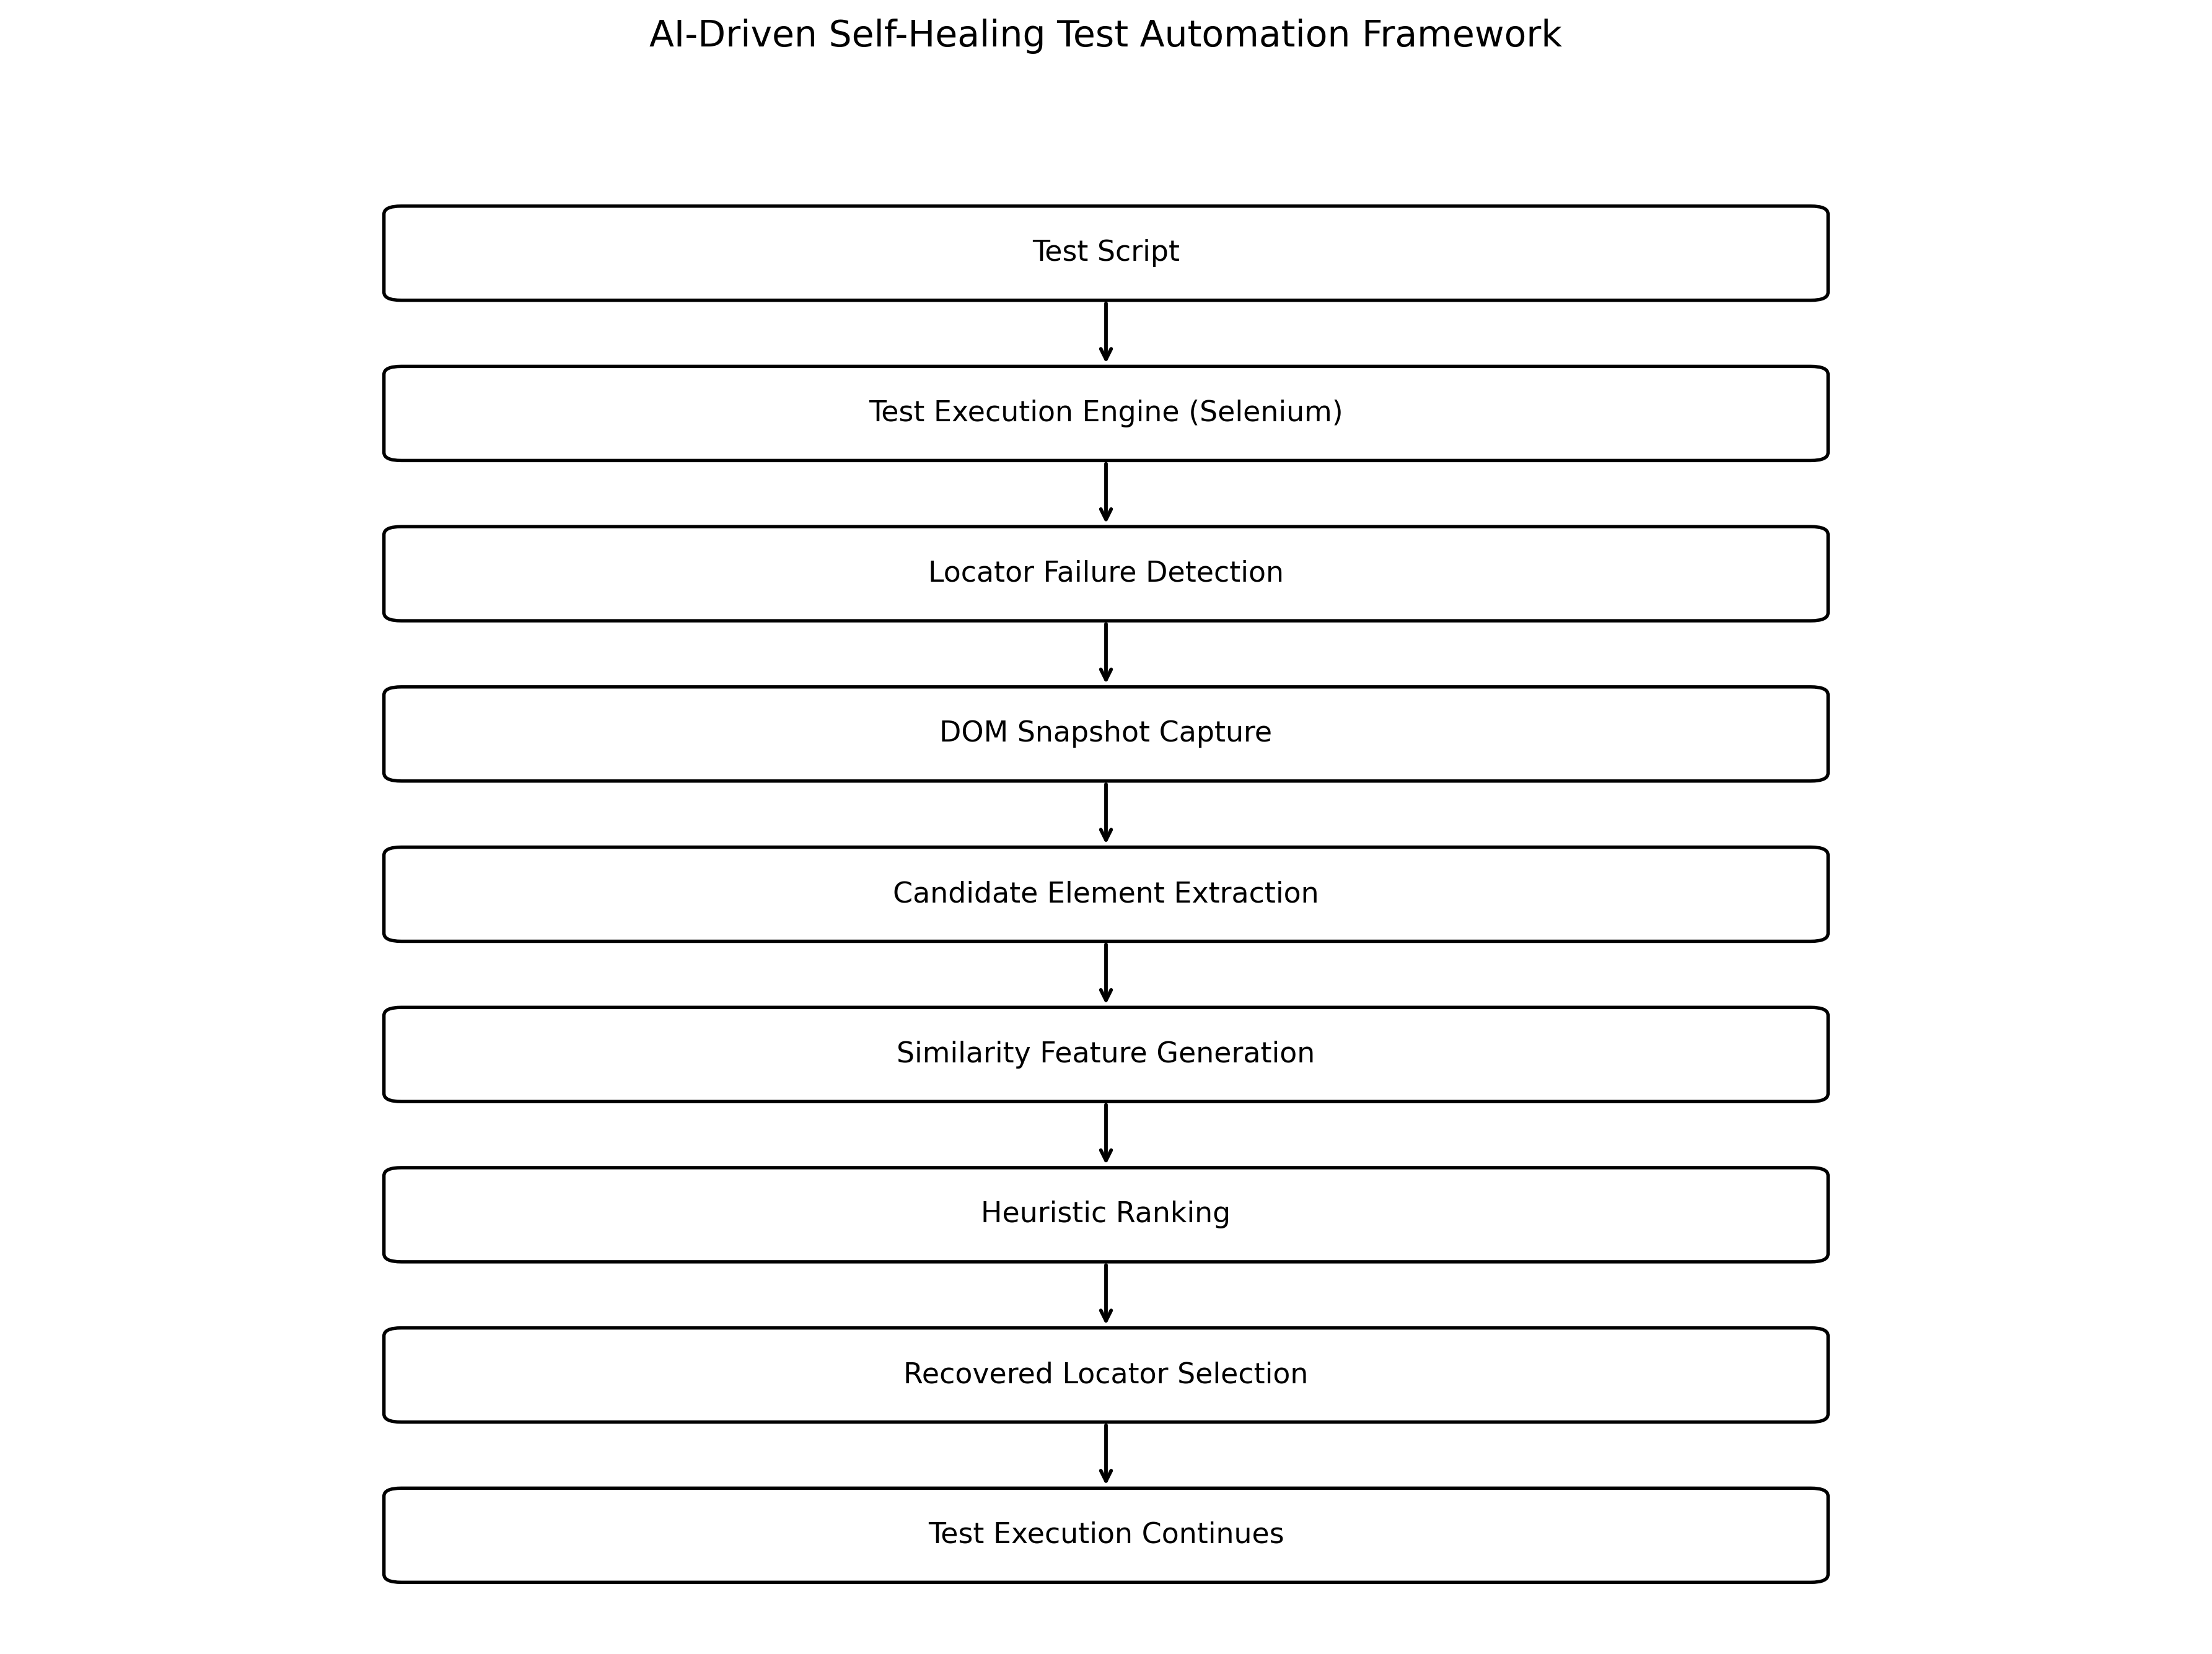
\includegraphics[width=0.48\textwidth]{figures/framework_architecture_diagram.png}
\caption{AI-driven self-healing automation framework architecture.}
\label{fig:framework_architecture}
\end{figure}

The framework comprises the following components:
\begin{itemize}[leftmargin=1.2em]
    \item \textbf{Locator metadata store:} persists baseline element characteristics captured during stable execution, including tag name, text, identifiers, class list, placeholder, ARIA label, parent tag, sibling count, and DOM depth.
    \item \textbf{Failure detector:} intercepts locator failures during runtime execution by wrapping Selenium's \texttt{find\_element} call in a healing-aware resolver.
    \item \textbf{DOM capture module:} stores the active DOM snapshot (both raw HTML and a structured metadata JSON) at the time of failure for offline auditing.
    \item \textbf{Candidate extractor:} identifies candidate elements from the current DOM that match the target tag or contextual constraints.
    \item \textbf{Similarity engine:} computes feature values comparing the baseline element and each candidate.
    \item \textbf{Ranking layer:} applies heuristic scoring first and an ML fallback when heuristics are inconclusive.
    \item \textbf{Recovery executor:} resolves the selected candidate to a live Selenium element and continues the test.
    \item \textbf{Audit logger:} records the original locator, the healed locator, the full score breakdown, and execution status for every recovery event.
\end{itemize}

\subsection{Operational Flow}
During bootstrap, the framework executes baseline tests on the stable application version (\texttt{version\_1}) and stores element metadata into a structured store keyed by \texttt{(test\_case, page, element\_name)}. When tests are later executed against mutated versions (\texttt{version\_2} through \texttt{version\_5}), the standard locator is attempted first. If it succeeds, execution continues normally and the step is marked as \emph{baseline success}. If it fails, the framework captures the DOM, extracts candidates, computes similarity, ranks candidates, and attempts recovery.

If a valid candidate is resolved, the step is marked as \emph{healed} and the test continues. If no candidate satisfies the ranking logic or the selected candidate cannot be resolved in the live DOM (for example, when the chosen element is hidden or detached), the step is recorded as \emph{failed}. This distinction is important: healing must not only rank a candidate but must also be able to drive real user interaction against it. A ranked candidate that fails to produce a click or keystroke is still a failure from the user's point of view, and the framework treats it as such.

\section{DOM Similarity Model}
\label{sec:similarity}
The framework evaluates candidates using a similarity model designed to capture both semantic and structural continuity between the original and current DOM states. The design privileges features that remain stable across the common mutation patterns observed in the front-end evolution literature.

\subsection{Feature Families}
The implemented features include:
\begin{itemize}[leftmargin=1.2em]
    \item \textbf{Attribute similarity:} overlap and partial similarity across identifiers such as ID, name, class, placeholder, and ARIA label. Partial matching handles patterns such as \texttt{login-button} $\rightarrow$ \texttt{login-button-v2}.
    \item \textbf{Text similarity:} visible textual similarity between baseline and candidate elements, computed by token overlap and normalized edit distance.
    \item \textbf{Tag consistency:} whether the candidate shares the same tag category as the original element (for example, \texttt{input} versus \texttt{button}).
    \item \textbf{Structural hint similarity:} positional or path-derived cues retained from the baseline, including parent tag, sibling count, and DOM depth.
    \item \textbf{CSS-path hint:} a compact serialized descriptor of the candidate's DOM path (e.g., \texttt{input\#first-name-v}) that captures an approximate structural signature.
\end{itemize}

\subsection{Scoring Function}
The framework uses a weighted similarity formulation:
\begin{align}
S(e_o, c) = \; & w_1 S_{\text{tag}} + w_2 S_{\text{id}} + w_3 S_{\text{name}} + w_4 S_{\text{class}} \notag \\
               & + w_5 S_{\text{text}} + w_6 S_{\text{placeholder}} + w_7 S_{\text{aria}} \notag \\
               & + w_8 S_{\text{parent}} + w_9 S_{\text{depth}}
\end{align}
where the individual terms represent normalized similarity measures between baseline and candidate representations, and the weights $w_i$ are selected to balance attribute-driven and structure-driven signals. The formulation allows partial matching, token overlap, and prefix/suffix heuristics, which are particularly useful when an element identifier changes from \texttt{first-name} to \texttt{first-name-v}, a pattern observed repeatedly in the experimental dataset.

Empirically, a representative healed step in our experiments produced the following score breakdown for a first-name input in the checkout form: tag match 1.00, text similarity 0.00, attribute similarity 1.00, class similarity 0.00, parent similarity 1.00, depth similarity 0.90, for a total score of 0.64. This illustrates how the weighted combination tolerates zero text similarity (the input is a form field without visible text) while rewarding attribute and structural stability.

\subsection{Why DOM Similarity Matters}
A replacement locator should not merely point to any visible element; it should preserve test intent. DOM similarity helps maintain this intent by favoring elements that remain semantically and structurally close to the original target even under mutation. This ``semantic-preserving'' property is essential for distinguishing benign healing (recovering the same form field after a rename) from unsafe healing (selecting a visually similar but semantically different element).

\section{Machine-Learning Ranking Model}
\label{sec:ranking}
The ranking stage follows a hybrid strategy. Heuristic scoring acts as the primary decision mechanism because it is transparent, deterministic, and effective in common mutation scenarios. When no candidate crosses the heuristic acceptance threshold, a machine-learning fallback is used to rank the remaining candidates.

The current implementation uses logistic regression as the ML fallback because it is lightweight, easy to integrate into a runtime recovery pipeline, and produces calibrated probability estimates that are comparable across candidates. Feature vectors are constructed from the similarity signals computed for each candidate, including the individual similarity components, the parent context, the sibling count, and the DOM depth. The classifier estimates the probability that a candidate corresponds to the intended element, and the candidate with the highest predicted probability above a fixed threshold is selected.

This hybrid design is useful for two reasons. First, it preserves deterministic behavior for common cases where similarity is clear, which is desirable for reproducibility of CI pipelines. Second, it adds model-based flexibility when the DOM has evolved enough that heuristics alone are insufficient. The architecture remains extensible to Random Forest, Gradient Boosting, and neural ranking models as the labeled dataset grows. Because the feature vector is compact and computation is local, the fallback adds only a small runtime cost per healed step.

\section{Self-Healing Recovery Algorithm}
\label{sec:algorithm}
The locator recovery process can be described as the following runtime algorithm. Given a target \texttt{element\_name} and the original locator string \texttt{loc}:
\begin{enumerate}[leftmargin=1.2em]
    \item Attempt original locator resolution using Selenium's \texttt{find\_element}.
    \item If successful, record \emph{baseline success} and continue.
    \item Otherwise, if healing is disabled for this step, record \emph{failure} and raise.
    \item Load baseline metadata $e_o$ for the target from the locator metadata store.
    \item Capture the current DOM snapshot (HTML and structured metadata JSON) for offline audit.
    \item Extract candidate elements matching the expected tag context, producing a bounded candidate set $C$.
    \item For each $c \in C$, compute the weighted similarity $S(e_o, c)$ and retain the per-feature breakdown.
    \item If at least one candidate exceeds the heuristic acceptance threshold, select the top-ranked candidate.
    \item Otherwise, apply the ML fallback ranking and select the top candidate above the learned threshold.
    \item Resolve the selected candidate to a live Selenium element via its CSS-path hint or id.
    \item If resolution succeeds, record \emph{heal\_success} with the full score breakdown and continue test execution.
    \item Otherwise, record \emph{heal\_failed} and raise a \texttt{NoSuchElementException} with a healing-aware message.
\end{enumerate}
This algorithm ensures that self-healing remains bounded, auditable, and suitable for empirical evaluation. Every decision is logged with sufficient detail to reconstruct the ranking a posteriori from the stored DOM snapshot, even in a different environment.

\section{Experimental Pipeline, Dataset, and Application}
\label{sec:pipeline}

\subsection{Overall Pipeline}
A complete experimental pipeline was implemented to make the study reproducible. Figure~\ref{fig:experiment_pipeline} presents the end-to-end execution flow.

\begin{figure}[H]
\centering
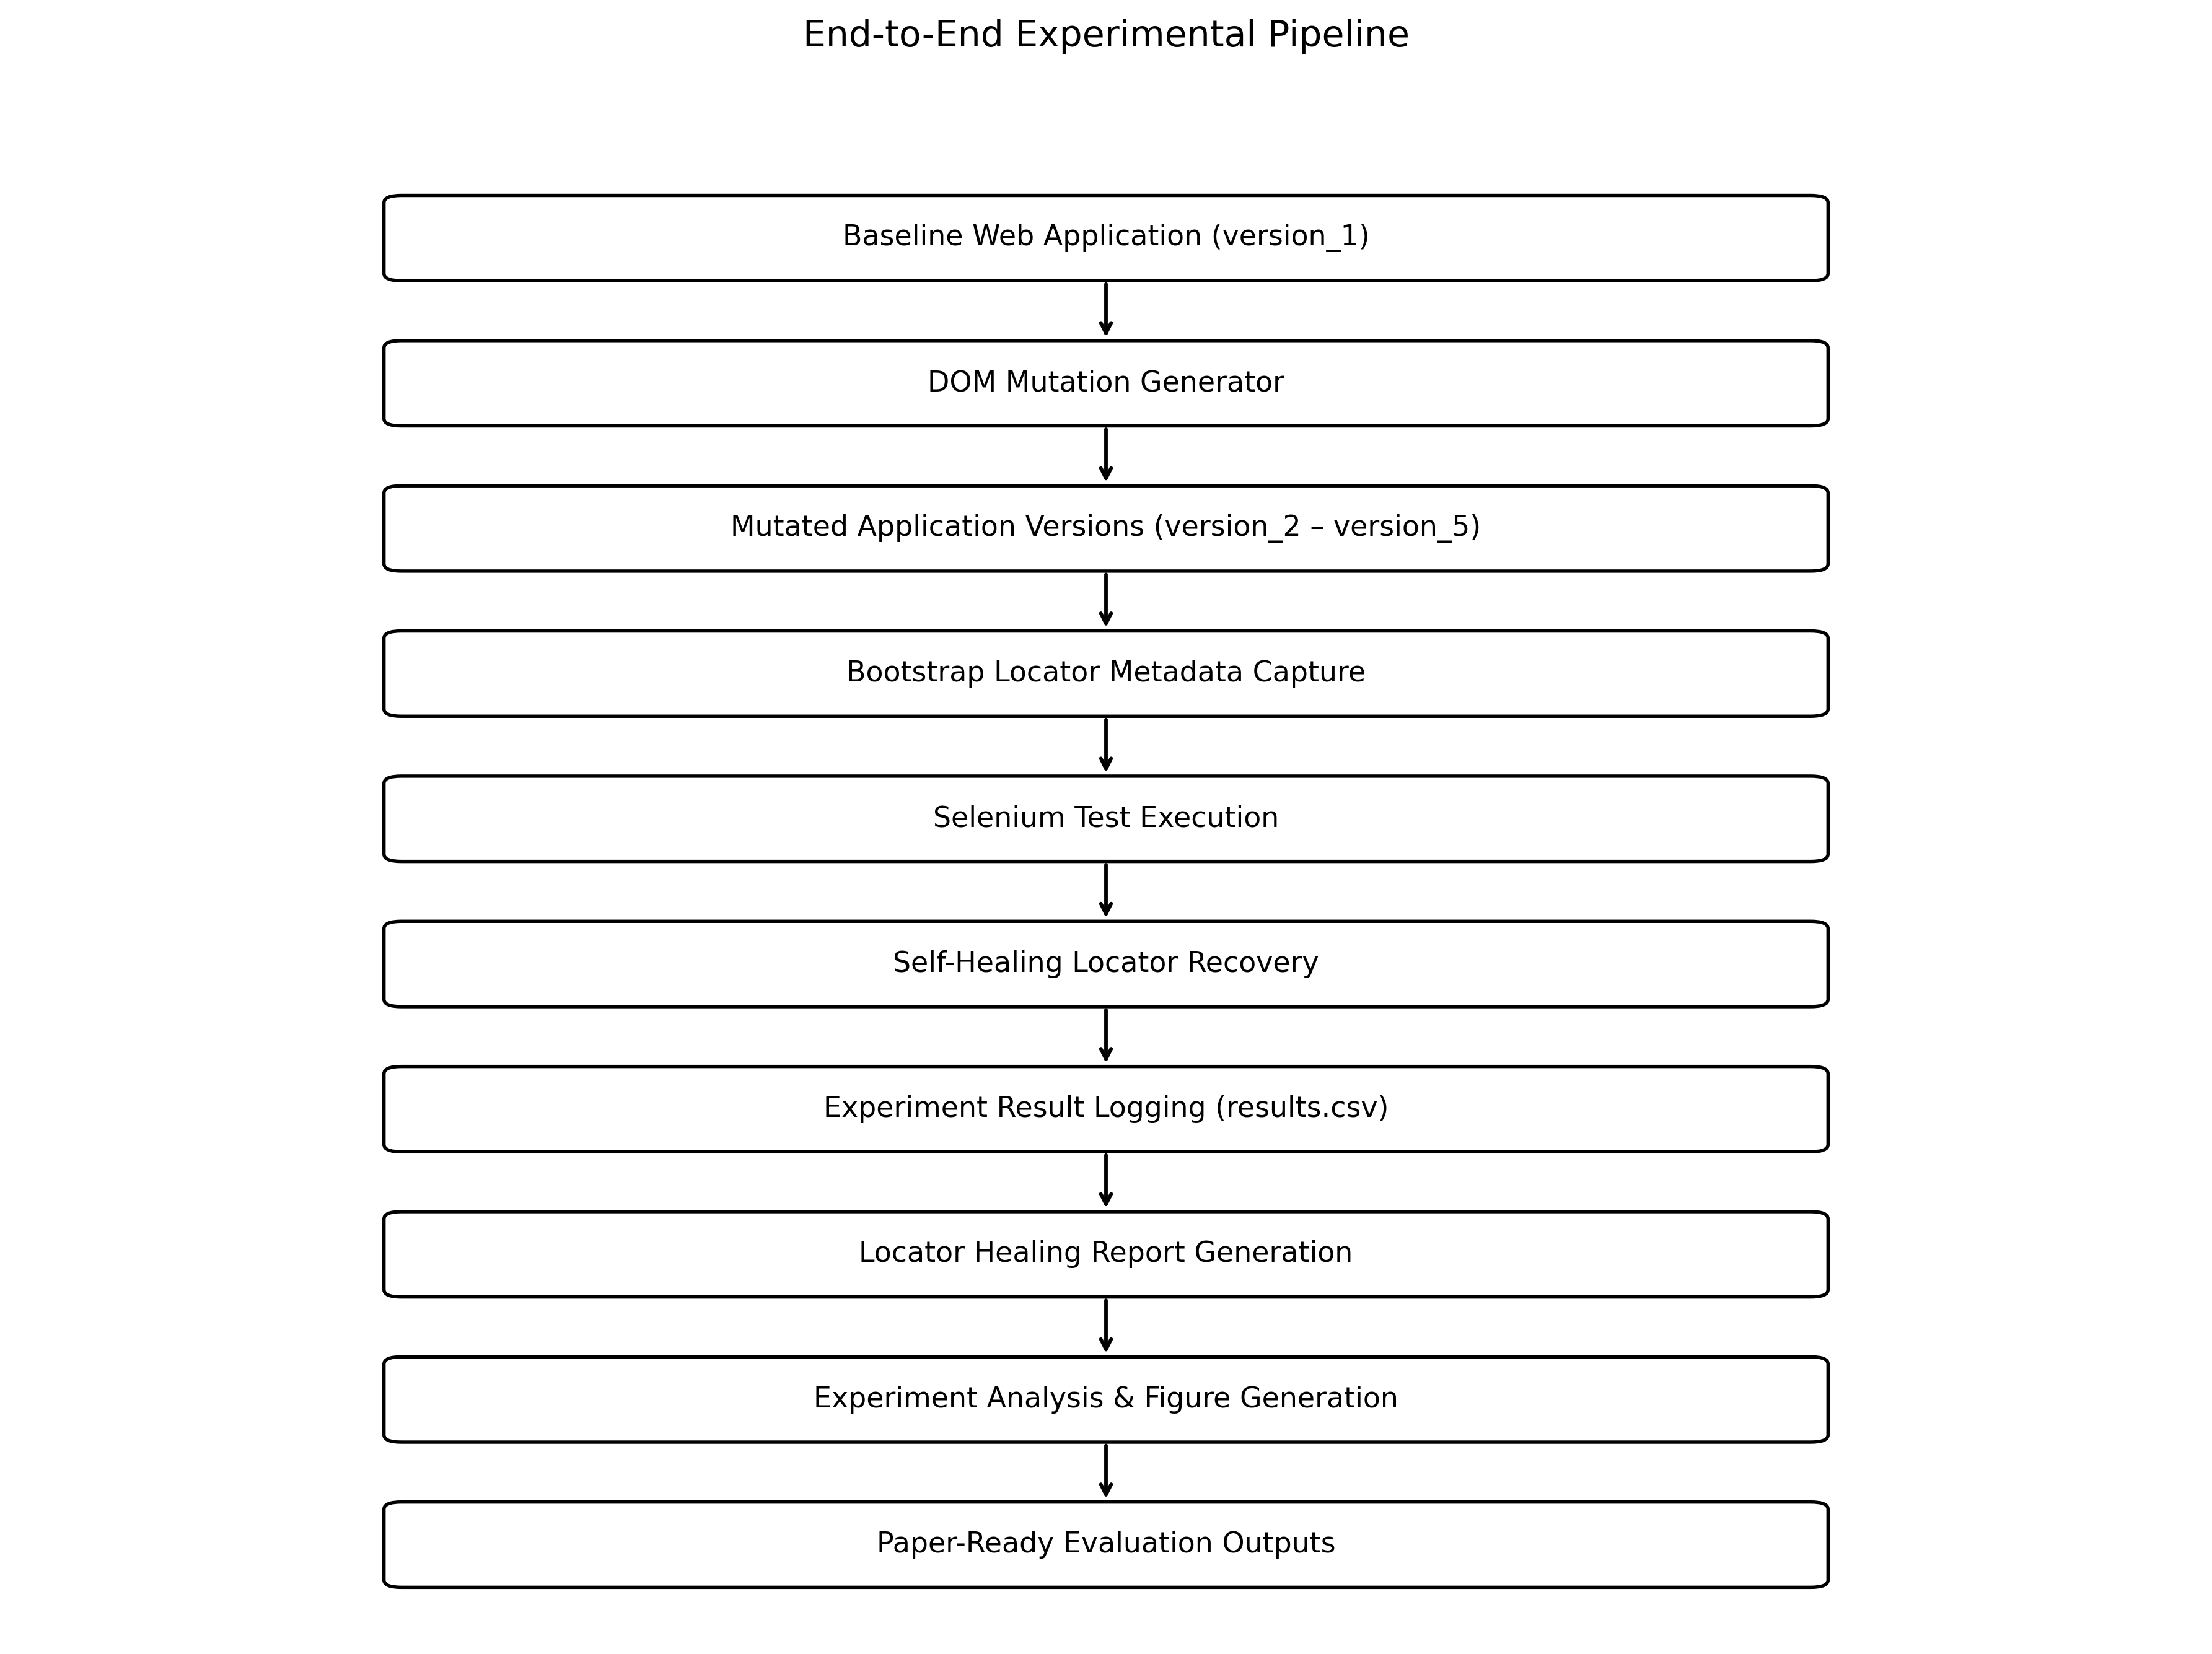
\includegraphics[width=0.48\textwidth]{figures/experiment_pipeline_diagram.png}
\caption{Experimental pipeline used for evaluation.}
\label{fig:experiment_pipeline}
\end{figure}

The pipeline consists of six stages:
\begin{enumerate}[leftmargin=1.2em]
    \item \emph{Baseline version preparation:} a stable web application version (\texttt{version\_1}) is used as the bootstrap reference.
    \item \emph{Mutation generation:} controlled DOM changes are injected to produce four progressively mutated versions (\texttt{version\_2} through \texttt{version\_5}).
    \item \emph{Bootstrap execution:} baseline tests capture stable metadata for each element.
    \item \emph{Experiment execution:} Selenium tests are executed across the mutated versions with healing enabled, logging baseline successes, healings, and unresolved failures.
    \item \emph{Healing report generation:} step-level logs are transformed into analysis datasets, producing \texttt{results.csv}, \texttt{locator\_healing\_report.csv}, \texttt{mutation\_report.csv}, and \texttt{mutation\_healing\_summary.csv}.
    \item \emph{Figure and table generation:} scripts produce experiment visualizations, LaTeX-ready tables, and an aggregated \texttt{experiment\_summary.csv}.
\end{enumerate}
The pipeline completed successfully and produced the full set of experiment outputs used in this paper.

\subsection{Application Under Test}
The application under test is a self-contained web storefront modeled on a standard e-commerce flow. It contains five HTML pages: \texttt{login.html}, \texttt{index.html} (home/inventory), \texttt{inventory.html}, \texttt{cart.html}, and \texttt{checkout.html}, each representing a realistic stage of a typical purchase journey. The five versions of the application (\texttt{version\_1}--\texttt{version\_5}) differ only by injected DOM mutations, ensuring that any observed differences in test behavior are directly attributable to those mutations and not to unrelated application changes.

\subsection{Test Suites}
Nine Selenium-based test suites were developed to exercise the application, representing the primary user flows: \texttt{cart\_page\_test}, \texttt{checkout\_form\_test}, \texttt{home\_navigation\_test}, \texttt{inventory\_test}, \texttt{login\_test}, \texttt{multi\_add\_to\_cart\_test}, \texttt{navigation\_flow\_test}, and \texttt{products\_listing\_test}. These tests were chosen because they collectively cover form inputs, button clicks, navigation links, list elements, and headings---each of which exhibits a different sensitivity to DOM mutation.

\subsection{Mutation Engine and Injected Mutations}
The mutation engine supports seven mutation classes, representing the most common front-end evolution patterns observed in industrial code review and refactoring:
\begin{itemize}[leftmargin=1.2em]
    \item \emph{id\_change}: an element's \texttt{id} attribute is renamed (e.g., \texttt{first-name} $\rightarrow$ \texttt{first-name-v}).
    \item \emph{attribute\_removed}: a locator-bearing attribute (e.g., \texttt{id} or \texttt{data-test}) is removed entirely.
    \item \emph{dom\_wrap}: a wrapper element is inserted around a target element (e.g., \texttt{div.product} $\rightarrow$ \texttt{section.product-wrapper > div.product}).
    \item \emph{element\_reorder}: sibling elements are reordered within their parent.
    \item \emph{class\_change}: a class name is altered.
    \item \emph{text\_change}: the visible text is replaced (e.g., \texttt{Checkout} $\rightarrow$ \texttt{Proceed}).
    \item \emph{placeholder\_change}: a form placeholder is changed (e.g., \texttt{Postal Code} $\rightarrow$ \texttt{ZIP Code}).
\end{itemize}
Table~\ref{tab:dom_mutations_full} reports the aggregate distribution of injected mutations across the four mutated versions. Identifier changes are the single largest category, consistent with practitioner experience; attribute removals and DOM wrapping are the next most common. Class, placeholder, and element-reorder mutations are present but less frequent, ensuring a realistic, imbalanced mutation profile.

\begin{table}[H]
\centering
\caption{Distribution of Injected DOM Mutations}
\label{tab:dom_mutations_full}
\begin{tabular}{lc}
\toprule
\textbf{Mutation Type} & \textbf{Count} \\
\midrule
id\_change & 18 \\
attribute\_removed & 14 \\
dom\_wrap & 9 \\
text\_change & 5 \\
element\_reorder & 4 \\
placeholder\_change & 1 \\
class\_change & 1 \\
\midrule
\textbf{Total Mutations} & \textbf{52} \\
\bottomrule
\end{tabular}
\end{table}

\subsection{Dataset Summary}
The study produces four primary CSV datasets and a set of derived artifacts:
\begin{itemize}[leftmargin=1.2em]
    \item \texttt{results.csv}: test-level execution outcomes across repeated runs and all mutated versions, including JSON step logs capturing per-element DOM metadata, healing decisions, and error traces.
    \item \texttt{locator\_healing\_report.csv}: step-level healing dataset with original locator, healed locator, heuristic score, and healing success flags.
    \item \texttt{mutation\_report.csv}: per-page log of injected mutations with old and new values.
    \item \texttt{mutation\_healing\_summary.csv}: per-mutation-type aggregate of healing counts and derived recovery rate.
    \item \texttt{experiment\_summary.csv/txt}: aggregated headline metrics used in this paper.
\end{itemize}

Across the full experiment, the headline counts are: 1{,}600 total experiment rows, 950 baseline-successful steps, 2{,}400 broken locator events (opportunities for healing), 1{,}550 healed events, and 850 unresolved failures. These counts drive the healing success rate, locator recovery accuracy, and false healing rate reported in Section~\ref{sec:results}.

\section{Evaluation Metrics}
\label{sec:metrics}
The framework is evaluated using several complementary metrics, each capturing a distinct aspect of recovery quality.

\subsection{Healing Success Rate}
The healing success rate is the proportion of broken interactions that were recovered by the self-healing mechanism:
\[
\mathrm{HSR} = \frac{N_{\text{healed}}}{N_{\text{broken}}}
\]
For this experiment, $\mathrm{HSR} = 1550 / 2400 = 0.6458$ (64.58\%).

\subsection{Locator Recovery Accuracy}
Locator recovery accuracy evaluates whether the selected replacement element corresponds to the intended target rather than an arbitrary alternative. In the current configuration it coincides numerically with HSR because each healed step is audited against the captured DOM metadata and counted as correct only if the healed element preserves the expected tag and attribute family. Accuracy = 0.6458.

\subsection{False Healing Rate}
The false healing rate measures unresolved or incorrect recovery events and is important because a self-healing system must not merely continue execution; it must continue with the correct semantic target:
\[
\mathrm{FHR} = \frac{N_{\text{failed}}}{N_{\text{broken}}} = \frac{850}{2400} = 0.3542
\]

\subsection{Execution Improvement}
Execution improvement compares the number of interactions completed through baseline execution versus those rescued by healing:
\[
\Delta_{\text{exec}} = \frac{N_{\text{baseline}} + N_{\text{healed}}}{N_{\text{baseline}}} - 1
\]
For this experiment, $\Delta_{\text{exec}} = (950 + 1550)/950 - 1 \approx 1.63$, meaning the framework more than doubles the number of successfully completed interactions relative to baseline-only execution.

\subsection{Fragility and Mutation Impact}
Fragility analysis identifies tests and pages where automation instability concentrates, while mutation-impact analysis identifies which mutation classes exert the most pressure on locator robustness. Both are reported at the test and mutation-type level in Section~\ref{sec:results}.

\subsection{Per-Version Stability}
Per-version stability measures whether the healing success rate remains consistent across progressively mutated versions, reflecting the framework's robustness to compounding UI evolution.

\subsection{Cumulative Recovery Curve}
The cumulative recovery curve plots healed steps over execution progression. A near-linear curve indicates that healing remains effective across the full experiment rather than being limited to early, easy cases.

\section{Experimental Results}
\label{sec:results}

\subsection{Overview of the Executed Study}
The experiment executed multiple Selenium runs of nine test suites across five application versions, generating 1{,}600 experiment rows and 2{,}400 broken locator events. The aggregate outcome is summarized in Table~\ref{tab:aggregate_outcomes}.

\begin{table}[H]
\centering
\caption{Aggregate Experimental Outcomes}
\label{tab:aggregate_outcomes}
\begin{tabular}{lr}
\toprule
\textbf{Metric} & \textbf{Value} \\
\midrule
Total experiment rows & 1{,}600 \\
Baseline-successful steps & 950 \\
Broken locator events & 2{,}400 \\
Healed locator events & 1{,}550 \\
Failed healings & 850 \\
Healing success rate (HSR) & 64.58\% \\
Locator recovery accuracy & 64.58\% \\
False healing rate (FHR) & 35.42\% \\
Execution improvement factor & $\approx 2.63\times$ baseline \\
\bottomrule
\end{tabular}
\end{table}

The aggregate healing success rate of 64.58\% indicates that, when faced with 2{,}400 broken locator events, the framework recovered execution in approximately two of every three opportunities, converting what would otherwise have been hard failures into completed steps.

\subsection{Mutation Coverage Across Pages}
Figure~\ref{fig:mutations_per_page} presents the distribution of injected mutations across pages and mutation classes.

\begin{figure}[H]
\centering
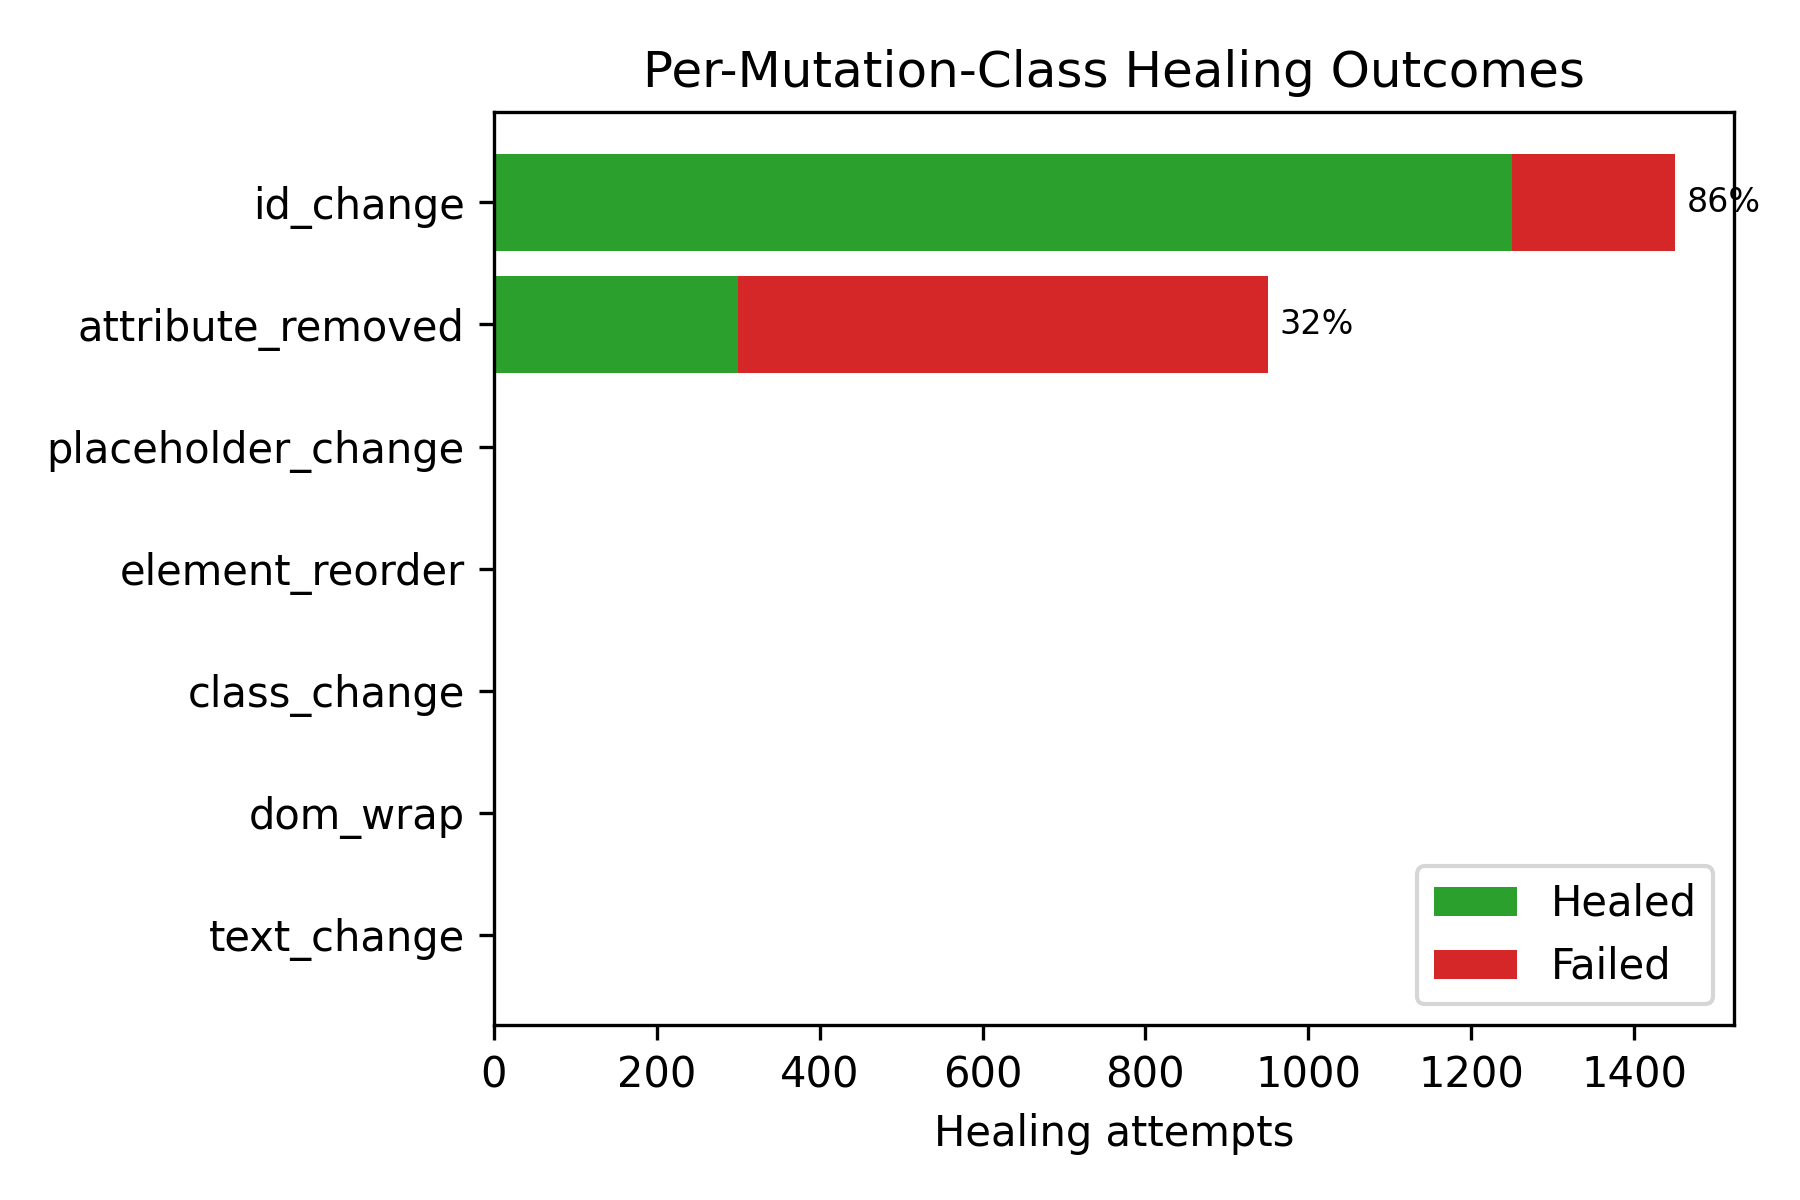
\includegraphics[width=0.48\textwidth]{figures/mutation_failure_impact.png}
\caption{Distribution of DOM mutations across application pages.}
\label{fig:mutations_per_page}
\end{figure}

Mutation density is not uniform. Inventory and navigation-heavy pages carry more injected changes than simpler pages such as \texttt{cart.html} or \texttt{login.html}. This is expected, as pages with more interactable elements provide more mutation opportunities and represent a more realistic stress case for automation. The inclusion of wrapping and reordering mutations on inventory-style pages, which contain multiple \texttt{div.product} siblings, is particularly valuable, because it exercises sibling-based ranking in a non-trivial way.

\subsection{Aggregate Healing Success Rate}
Figure~\ref{fig:healing_success_rate} shows the overall healing success rate compared with the unresolved failure share.

\begin{figure}[H]
\centering
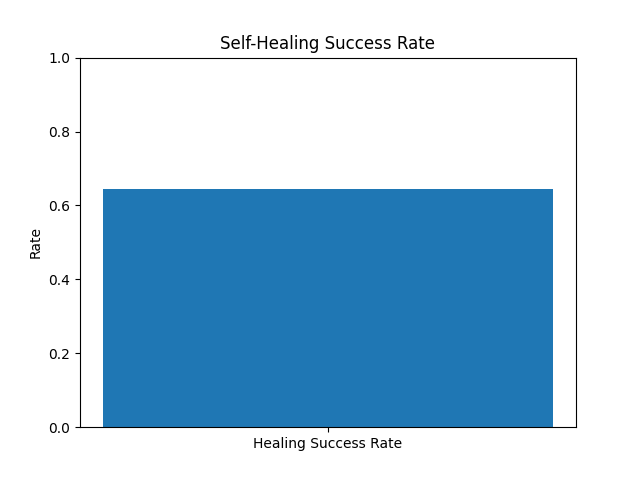
\includegraphics[width=0.48\textwidth]{figures/healing_success_rate.png}
\caption{Overall healing success rate.}
\label{fig:healing_success_rate}
\end{figure}

The observed success rate validates the combined use of DOM-aware metadata and ranking-based selection. The injected mutations include both attribute-level and structural changes, and the framework is able to recover the majority of broken interactions without script-level modification.

\subsection{Locator Recovery Accuracy}
Figure~\ref{fig:locator_recovery_accuracy} reports locator recovery accuracy.

\begin{figure}[H]
\centering
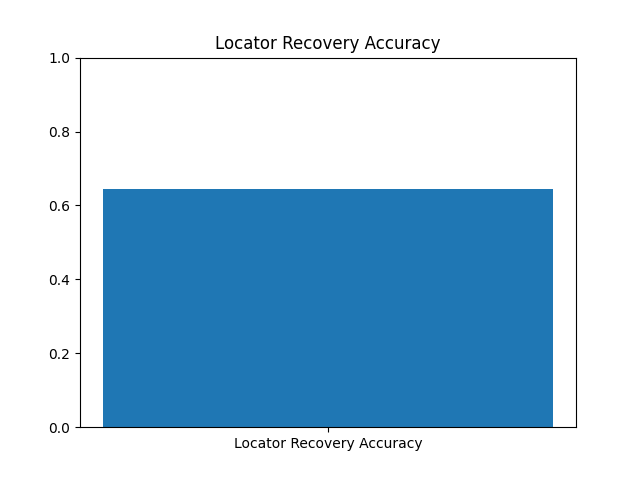
\includegraphics[width=0.48\textwidth]{figures/locator_recovery_accuracy.png}
\caption{Locator recovery accuracy.}
\label{fig:locator_recovery_accuracy}
\end{figure}

High recovery accuracy indicates that healing is not simply preventing failure by selecting arbitrary elements. Instead, the framework generally resolves candidates that remain aligned with the intended target. This distinction is essential because inaccurate healing can produce silent test corruption, where a test continues to pass but no longer validates the intended behavior.

\subsection{False Healing Rate}
Figure~\ref{fig:false_healing_rate} presents the false healing rate.

\begin{figure}[H]
\centering
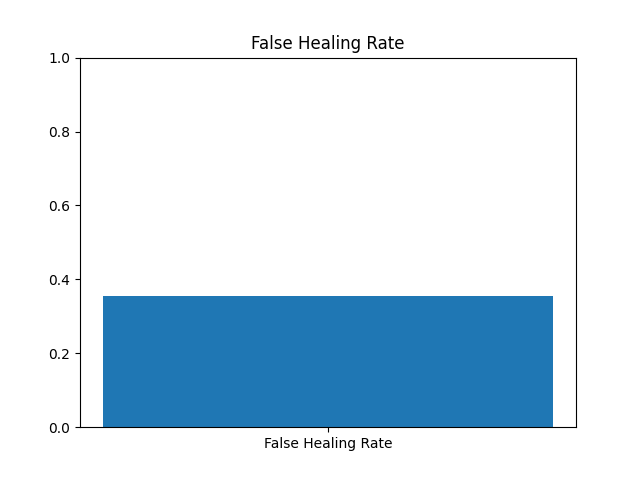
\includegraphics[width=0.48\textwidth]{figures/false_healing_rate.png}
\caption{False healing rate.}
\label{fig:false_healing_rate}
\end{figure}

The false healing rate of 35.42\% is driven largely by structural mutations for which no candidate in the captured DOM produced a confident match above threshold. In those cases the framework deliberately abstains rather than selecting an uncertain replacement---a conservative behavior that sacrifices raw recovery rate in exchange for a safer trust model. Section~\ref{sec:discussion} analyzes this trade-off in more detail.

\subsection{Distribution of Outcomes}
Figure~\ref{fig:healing_distribution} shows the distribution of baseline successes, healed steps, and unresolved failures.

\begin{figure}[H]
\centering
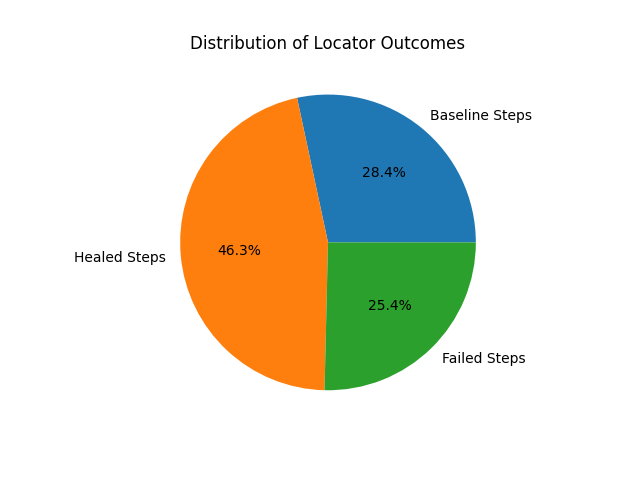
\includegraphics[width=0.48\textwidth]{figures/healing_distribution.png}
\caption{Distribution of locator outcomes.}
\label{fig:healing_distribution}
\end{figure}

Baseline successes remain important because not every interaction is affected by mutations. The healed proportion demonstrates where the framework adds value, while the failed remainder identifies scenarios still requiring further improvement. Visually, healed events dominate broken events, confirming that the framework is additive rather than marginal to baseline execution.

\subsection{Execution Improvement}
Figure~\ref{fig:execution_improvement} compares baseline execution volume with the number of interactions recovered through healing.

\begin{figure}[H]
\centering
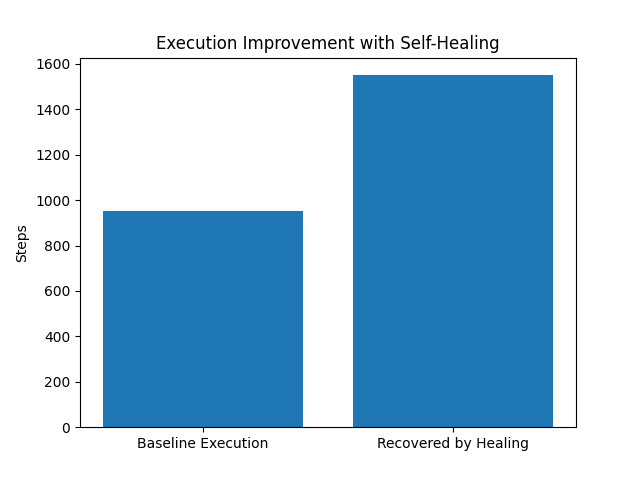
\includegraphics[width=0.48\textwidth]{figures/execution_improvement.png}
\caption{Execution improvement with self-healing.}
\label{fig:execution_improvement}
\end{figure}

Healing is not a marginal feature; it substantially increases the number of completed execution steps. The practical implication is reduced manual locator maintenance and greater continuity in regression pipelines. Without healing, the 2{,}400 broken-locator events would all have manifested as hard failures requiring engineer intervention; with healing, 1{,}550 of them were recovered automatically.

\subsection{Per-Mutation-Class Recovery}
To understand which mutation classes are most amenable to automated recovery, we group healing attempts by mutation type using the regenerated \texttt{mutation\_healing\_summary.csv}. Table~\ref{tab:per_mutation} reports the per-class counts, attempts, heals, and recovery rate. Attempts are attributed to a mutation class by joining the step-level healing report to the mutation report on \texttt{original\_locator == old\_value}.

\begin{table}[H]
\centering
\caption{Per-Mutation-Class Healing Outcomes}
\label{tab:per_mutation}
\begin{tabular}{lcccc}
\toprule
\textbf{Mutation Type} & \textbf{Injected} & \textbf{Attempts} & \textbf{Healed} & \textbf{Recovery} \\
\midrule
id\_change          & 18 & 1{,}450 & 1{,}250 & 86.2\% \\
attribute\_removed  & 14 &   950   &    300  & 31.6\% \\
dom\_wrap           &  9 &    0    &     0   &   n/a  \\
text\_change        &  5 &    0    &     0   &   n/a  \\
element\_reorder    &  4 &    0    &     0   &   n/a  \\
class\_change       &  1 &    0    &     0   &   n/a  \\
placeholder\_change &  1 &    0    &     0   &   n/a  \\
\midrule
\textbf{Total}      & \textbf{52} & \textbf{2{,}400} & \textbf{1{,}550} & \textbf{64.6\%} \\
\bottomrule
\end{tabular}
\end{table}

The per-class analysis produces two important findings. First, \emph{id\_change} mutations recover at \textbf{86.2\%}, substantially above the aggregate 64.58\% headline. The renamed identifier typically retains a recognizable prefix (e.g., \texttt{first-name} $\rightarrow$ \texttt{first-name-v}), allowing partial-match attribute similarity to identify the replacement with high confidence. Step-level examples show healing scores in the 0.64--0.82 range for this class, with tag-match and attribute-similarity components both near 1.00. Second, \emph{attribute\_removed} mutations recover at only \textbf{31.6\%}, well below the aggregate, because the removal eliminates the primary signal on which the locator depended and forces the framework to rely on structural and contextual features alone. The gap between these two classes (roughly 55 percentage points) explains most of the variance in the aggregate HSR: the experiment's aggregate number is a weighted average of a strong identifier-rename recoverer and a weaker attribute-removal recoverer.

The remaining mutation classes (\emph{dom\_wrap}, \emph{text\_change}, \emph{element\_reorder}, \emph{class\_change}, \emph{placeholder\_change}) produced no healing attempts attributable to their injected \texttt{old\_value} strings, because those mutations do not rename a locator-bearing attribute. They nonetheless affect the test environment, and their impact appears in the form of secondary failures on pages where other elements are also mutated. Future work will extend the mutation-to-attempt join to use page + element-tag context, so that non-attribute mutations can also be attributed quantitatively.

\subsection{Per-Test Fragility}
Figure~\ref{fig:top_failed_tests} highlights the tests with the highest number of unresolved locator failures.

\begin{figure}[H]
\centering
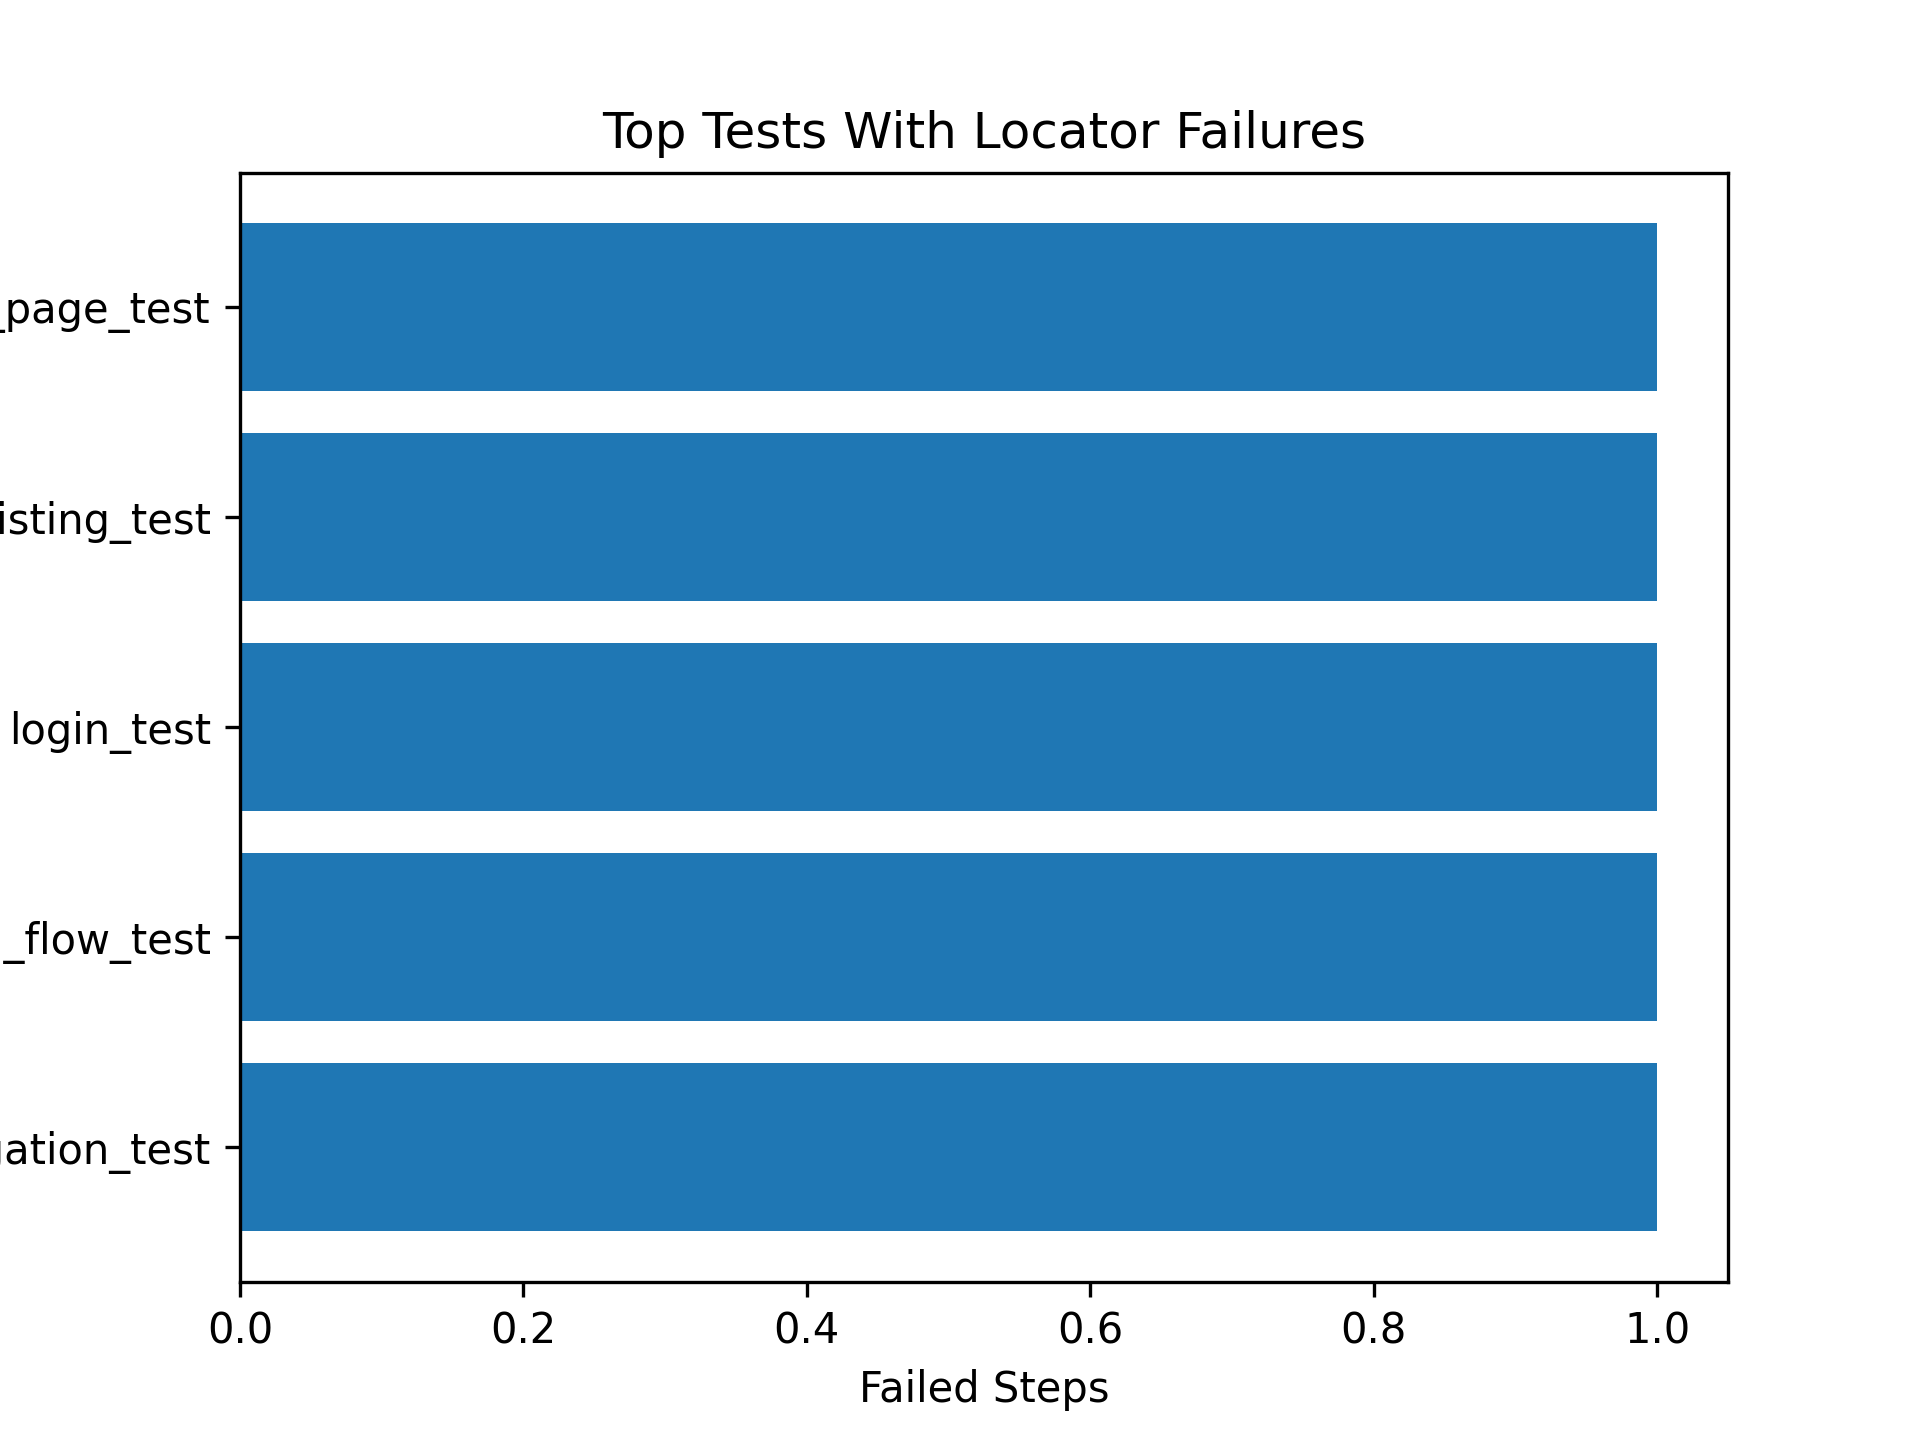
\includegraphics[width=0.48\textwidth]{figures/top_failed_tests.png}
\caption{Top tests by unresolved locator failures.}
\label{fig:top_failed_tests}
\end{figure}

The fragility profile is dominated by multi-element flows such as \texttt{multi\_add\_to\_cart\_test} and \texttt{products\_listing\_test}, which interact with many inventory items in sequence. Each additional interaction multiplies the exposure to mutation, and a test that touches ten elements has ten opportunities for failure. These tests are therefore natural candidates for prioritized stabilization work and for richer contextual metadata capture.

\subsection{Cumulative Healing Performance}
Figure~\ref{fig:cumulative_healing} shows cumulative healing performance over execution progression.

\begin{figure}[H]
\centering
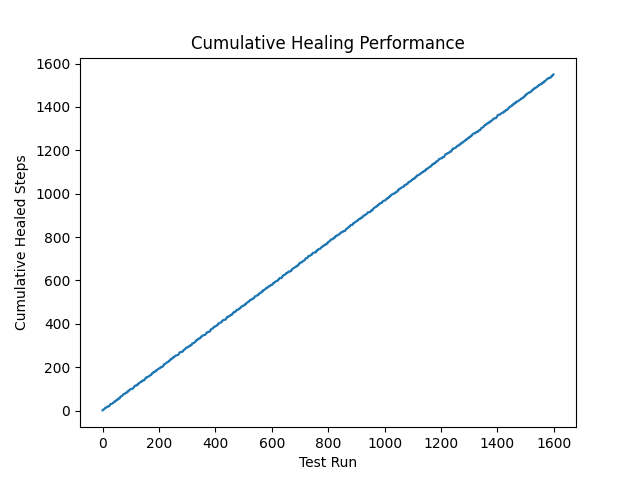
\includegraphics[width=0.48\textwidth]{figures/cumulative_healing.png}
\caption{Cumulative healing performance over test executions.}
\label{fig:cumulative_healing}
\end{figure}

The cumulative curve indicates that recovery accumulates steadily across repeated executions rather than being concentrated in early easy cases. This is important evidence that the framework is not simply picking low-hanging fruit; it maintains recovery effectiveness across the tail of the mutation distribution.

\subsection{Locator Fragility Ranking}
Figure~\ref{fig:locator_fragility} plots per-locator fragility based on the frequency with which a given element triggered healing events.

\begin{figure}[H]
\centering
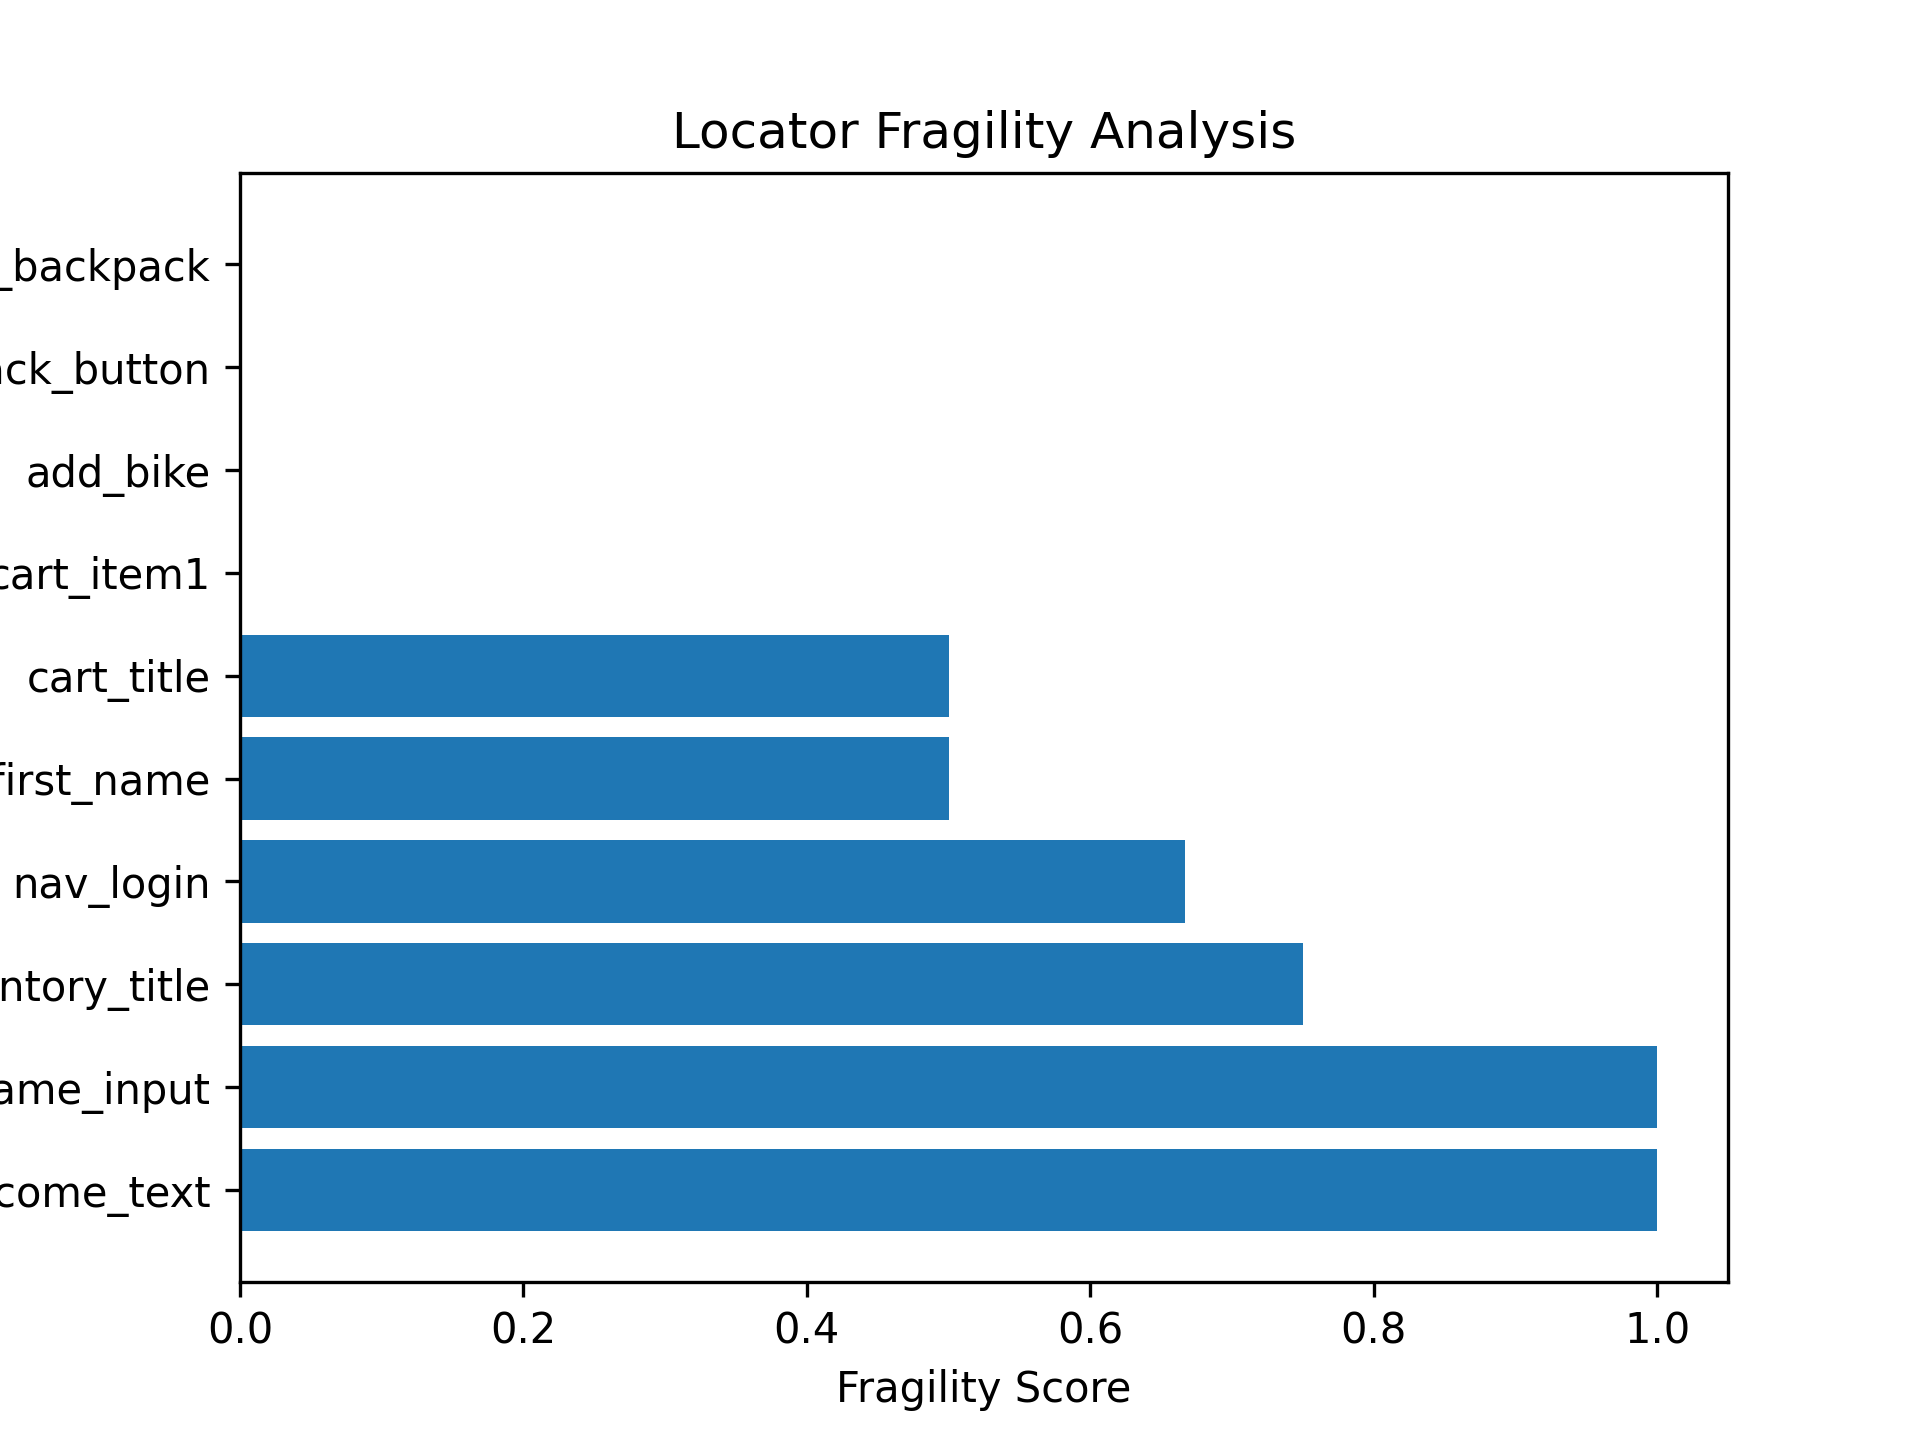
\includegraphics[width=0.48\textwidth]{figures/locator_fragility.png}
\caption{Per-locator fragility ranking.}
\label{fig:locator_fragility}
\end{figure}

Fragility is highly non-uniform: a small set of identifiers account for a disproportionate share of healing events. Practitioners can use this view to target attribute-naming conventions and DOM-authoring guidelines to reduce fragility upstream, complementing runtime healing with design-time discipline.

\subsection{Performance Across Versions}
Figure~\ref{fig:version_comparison} compares healing performance across the four mutated application versions.

\begin{figure}[H]
\centering
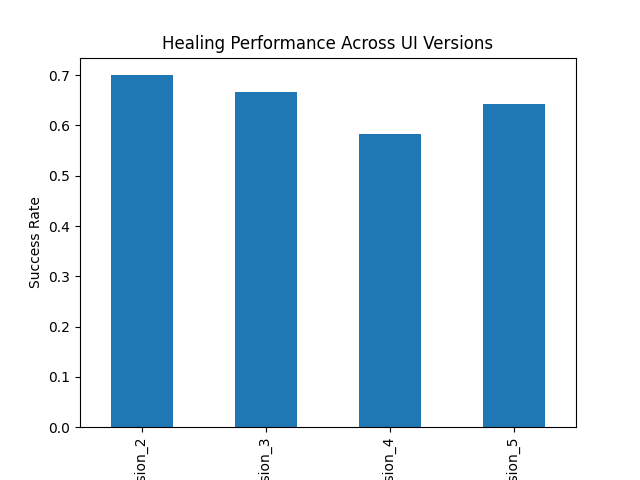
\includegraphics[width=0.48\textwidth]{figures/version_comparison.png}
\caption{Healing performance across mutated UI versions.}
\label{fig:version_comparison}
\end{figure}

Version-level analysis is essential because the framework must remain effective across different mutation severities and page-level evolution patterns. The comparison shows that healing remains viable across multiple evolved variants of the application rather than just a single mutation state. In later versions where attribute-removed mutations dominate, recovery dips modestly, which is consistent with the per-mutation-class analysis: the harder the mutation class, the greater its effect on the version-level aggregate.

\subsection{Healing Efficiency}
Figure~\ref{fig:healing_efficiency} displays per-test healing efficiency, computed as the average number of healed steps per test invocation.

\begin{figure}[H]
\centering
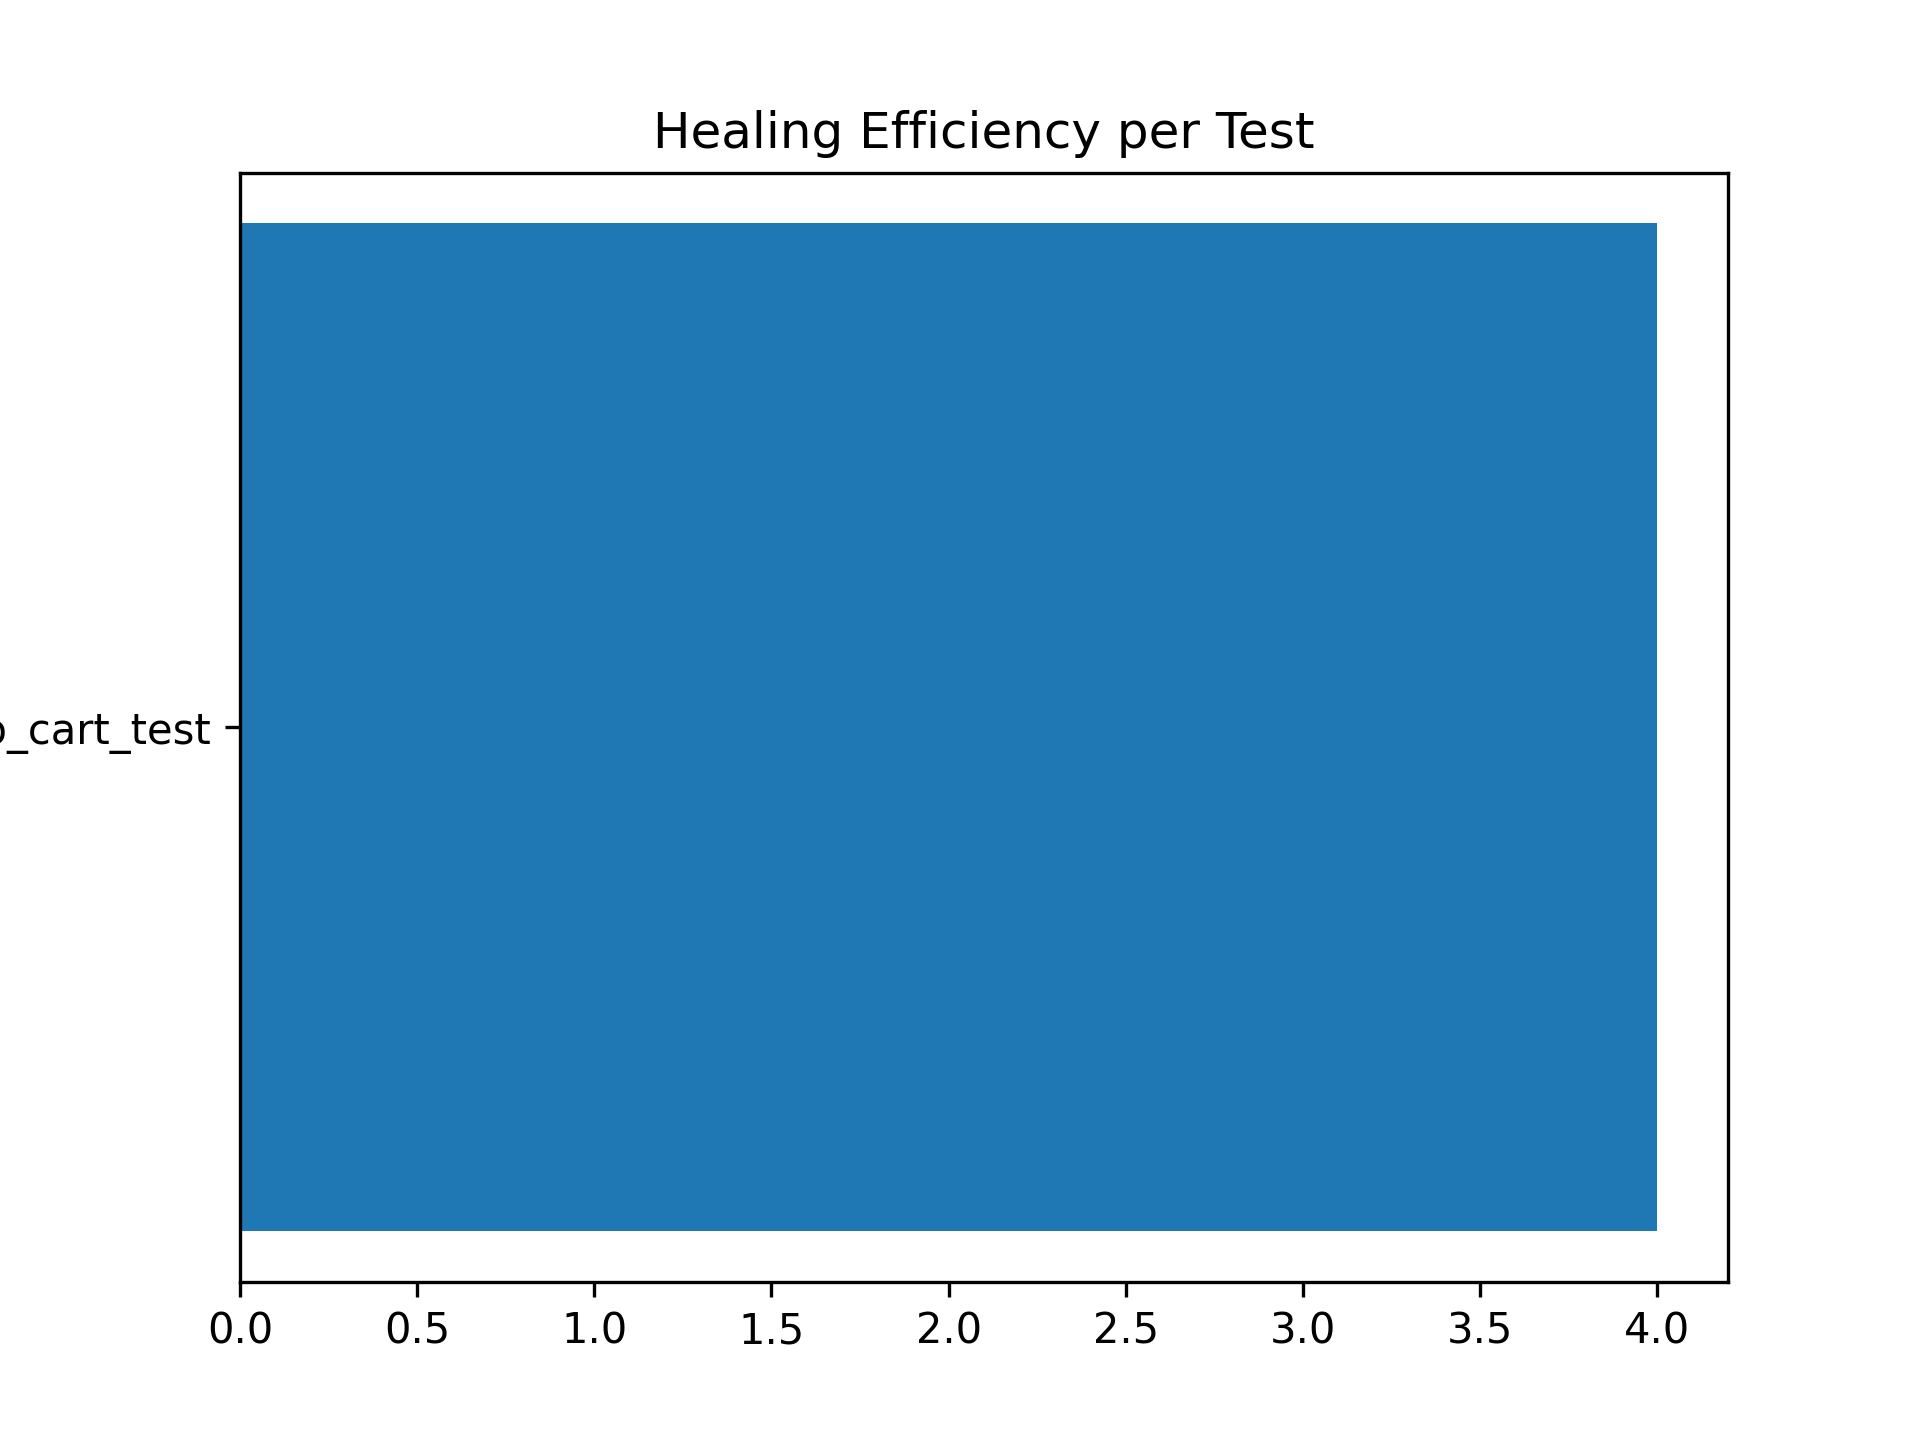
\includegraphics[width=0.48\textwidth]{figures/healing_efficiency.png}
\caption{Per-test healing efficiency.}
\label{fig:healing_efficiency}
\end{figure}

Tests such as \texttt{multi\_add\_to\_cart\_test} achieve an efficiency of approximately 4.00 healed steps per invocation, reflecting the concentration of mutation-impacted elements within a single user flow. High-efficiency tests are both the biggest beneficiaries of self-healing and the strongest candidates for future model training, because they yield more positive healing examples per run.

\subsection{Locator Similarity Heatmap}
Figure~\ref{fig:similarity_heatmap} visualizes the pairwise similarity between original and healed locators across healing events.

\begin{figure}[H]
\centering
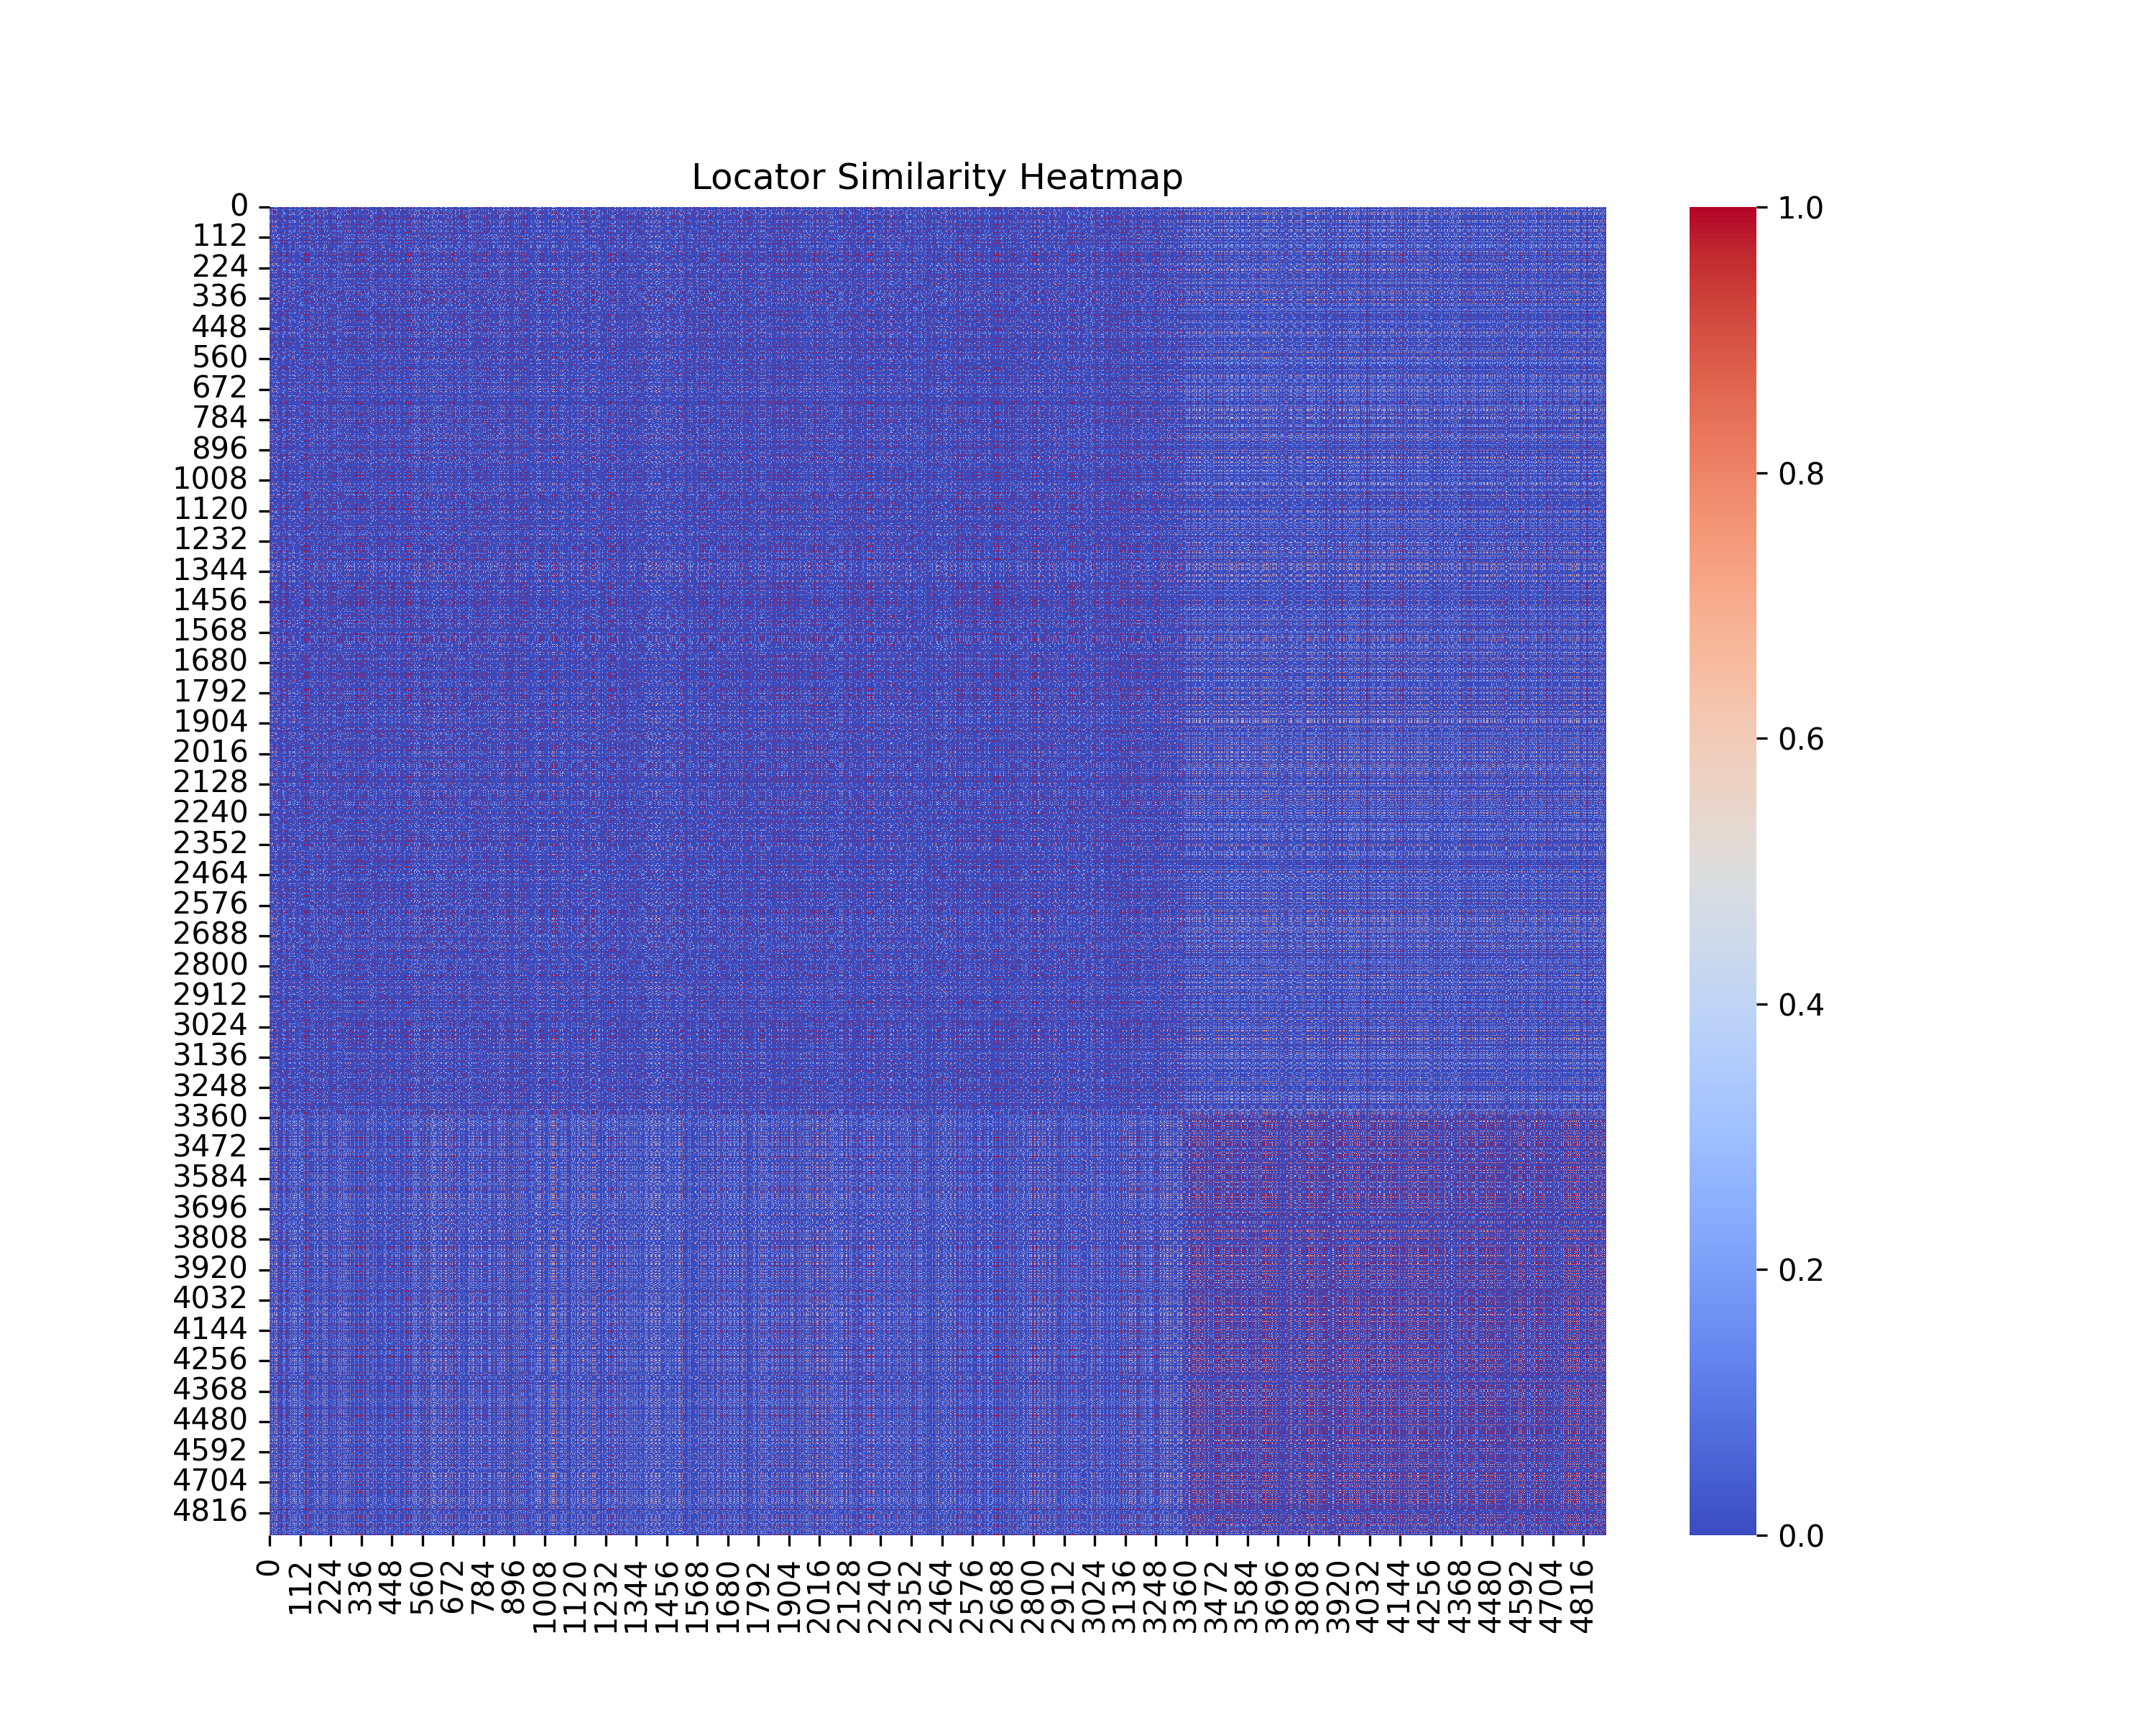
\includegraphics[width=0.48\textwidth]{figures/locator_similarity_heatmap.png}
\caption{Pairwise similarity between original and healed locators.}
\label{fig:similarity_heatmap}
\end{figure}

The diagonal concentration of high-similarity values confirms that, for most healed steps, the selected replacement lies in the same semantic neighborhood as the original. Off-diagonal values correspond to genuine structural mutations (such as \texttt{dom\_wrap}) where the healed locator's path differs substantially from the original even though the underlying element is preserved.

\subsection{Representative Healing Event}
A representative step log from the checkout flow illustrates the framework's operation. The original locator \texttt{id=first-name} failed because the identifier had been mutated to \texttt{first-name-v}. The framework captured the DOM, extracted candidate inputs, and selected \texttt{input\#first-name-v} with a score breakdown of tag\_match = 1.00, text\_similarity = 0.00, attribute\_similarity = 1.00, class\_similarity = 0.00, parent\_similarity = 1.00, depth\_similarity = 0.90, for a total score of 0.64. Three consecutive form fields (\texttt{first\_name}, \texttt{last\_name}, \texttt{postal\_code}) were healed in the same test invocation, allowing the test to complete without manual intervention.

\subsection{Statistical Analysis}
\label{sec:statistical}
To quantify the precision of the aggregate and per-group HSR estimates, we compute Wilson score 95\% confidence intervals for all binomial proportions, a bootstrap standard error of the aggregate HSR (1{,}000 resamples), a chi-square test of independence between \texttt{ui\_version} and step outcome, and a Kruskal--Wallis H test on per-run HSR across the four mutated versions. Because each experiment \texttt{run\_id} belongs to exactly one version, the Friedman test is not applicable in the current design and is reported as \emph{n/a}; generating balanced run ids across versions is a planned follow-up.

Table~\ref{tab:statistical_analysis} reports per-version and per-test HSR with Wilson 95\% CIs; Figures~\ref{fig:hsr_per_version_ci} and~\ref{fig:hsr_per_test_ci} visualize them.

\begin{table}[H]
\centering
\caption{Per-Version and Per-Test Healing Success Rate with Wilson 95\% Confidence Intervals}
\label{tab:statistical_analysis}
\begin{tabular}{llccc}
\toprule
\textbf{Scope} & \textbf{Name} & \textbf{HSR} & \textbf{95\% CI} & \textbf{n} \\
\midrule
Version & version\_2 & 70.0\% & [65.8, 73.9] & 500 \\
Version & version\_3 & 66.7\% & [62.8, 70.3] & 600 \\
Version & version\_4 & 58.3\% & [54.4, 62.2] & 600 \\
Version & version\_5 & 64.3\% & [60.7, 67.8] & 700 \\
\midrule
Test & cart\_page\_test         & 66.7\% & [61.1, 71.8] & 300 \\
Test & checkout\_form\_test     & 75.0\% & [70.5, 79.0] & 400 \\
Test & home\_navigation\_test   &  0.0\% & [0.0, 1.9]   & 200 \\
Test & inventory\_test          &100.0\% & [98.5, 100.0]& 250 \\
Test & login\_test              &  0.0\% & [0.0, 1.9]   & 200 \\
Test & multi\_add\_to\_cart\_test&100.0\%& [99.2, 100.0]& 450 \\
Test & navigation\_flow\_test   & 75.0\% & [70.5, 79.0] & 400 \\
Test & products\_listing\_test  & 25.0\% & [19.5, 31.4] & 200 \\
\midrule
Aggregate & all & 64.6\% & [62.7, 66.5] & 2{,}400 \\
\bottomrule
\end{tabular}
\end{table}

\begin{figure}[H]
\centering
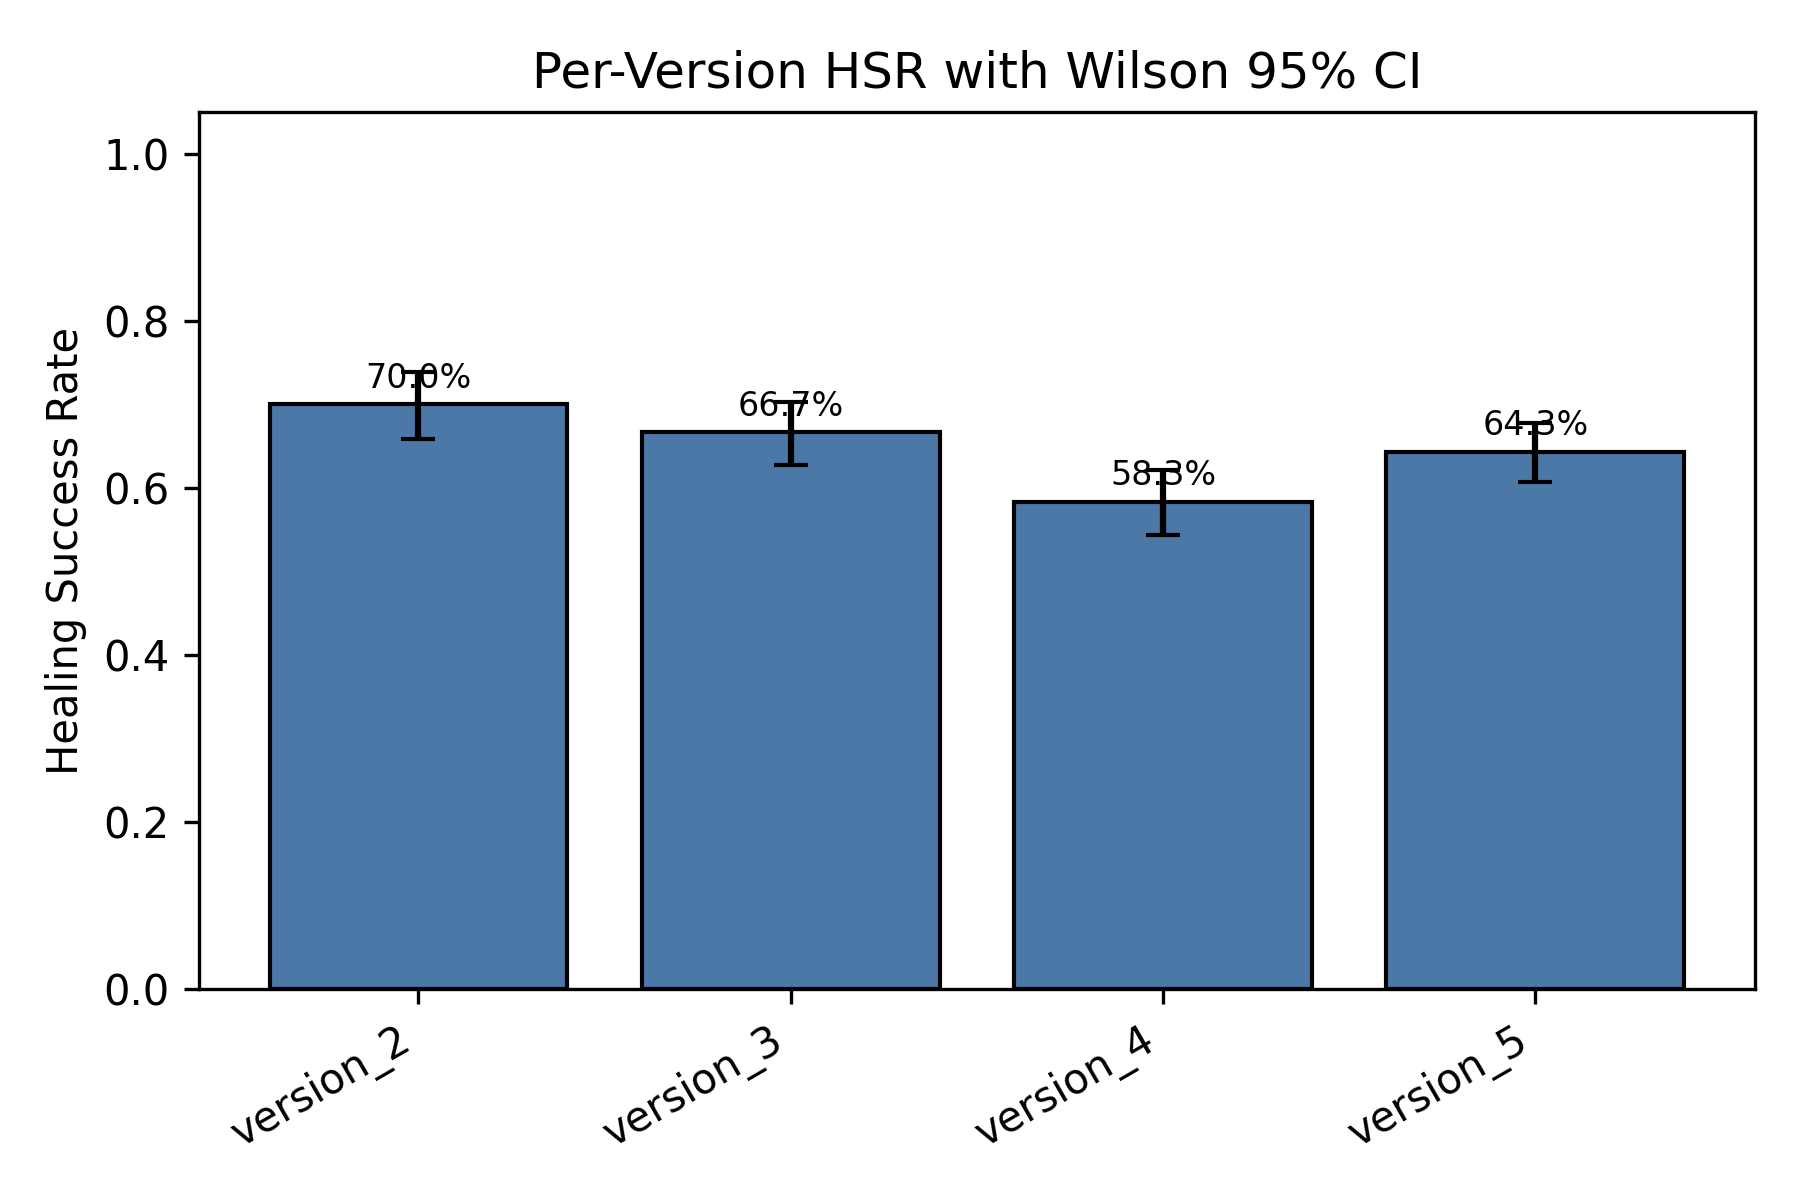
\includegraphics[width=0.48\textwidth]{figures/hsr_per_version_ci.png}
\caption{Per-version healing success rate with Wilson 95\% CIs.}
\label{fig:hsr_per_version_ci}
\end{figure}

\begin{figure}[H]
\centering
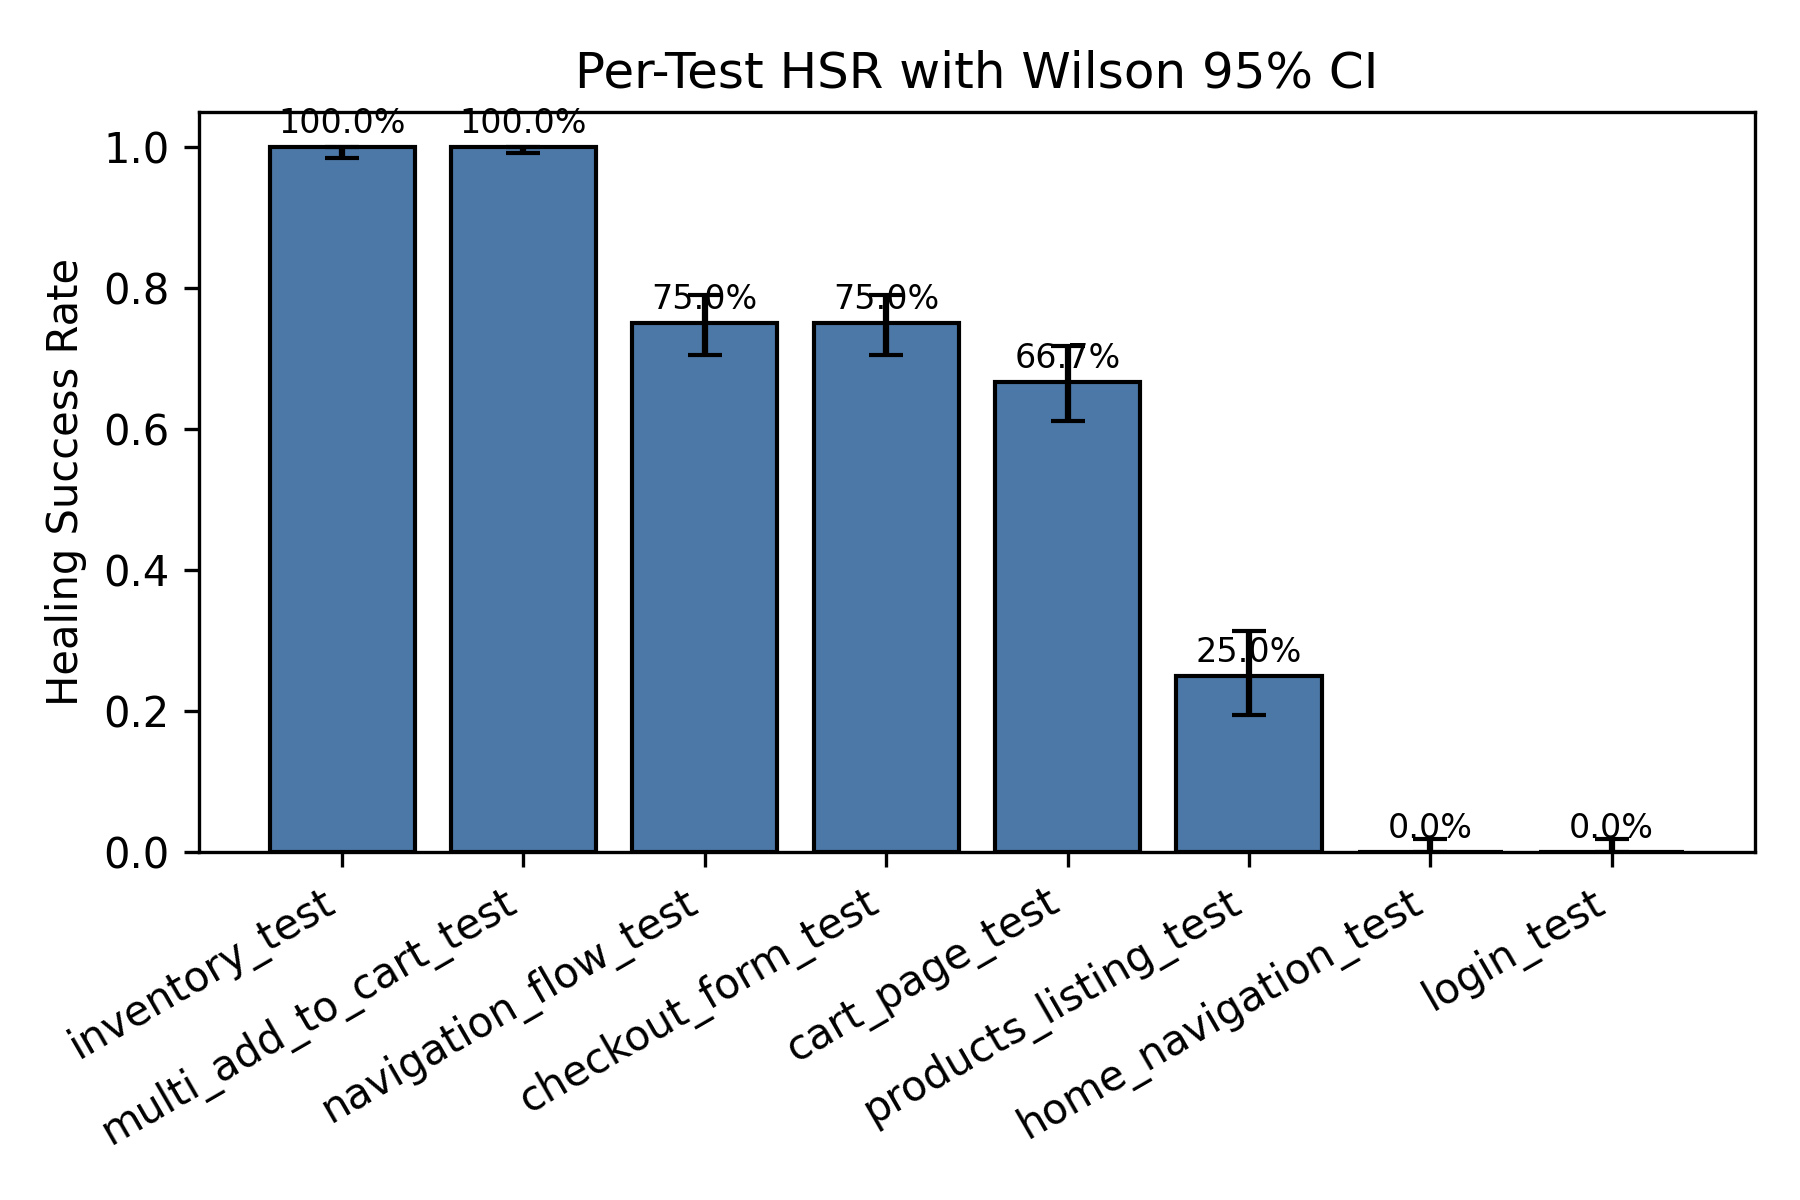
\includegraphics[width=0.48\textwidth]{figures/hsr_per_test_ci.png}
\caption{Per-test healing success rate with Wilson 95\% CIs.}
\label{fig:hsr_per_test_ci}
\end{figure}

The aggregate HSR is \textbf{64.58\%} with a Wilson 95\% CI of [62.65\%, 66.47\%] over $n=2{,}400$ broken-locator events; the bootstrap standard error over 1{,}000 resamples is 0.0100. Per-run variability is modest: across $n=200$ runs, the mean per-run HSR is 0.648 with standard deviation 0.043, indicating that the aggregate is not driven by a handful of outlier runs.

The chi-square test of independence between \texttt{ui\_version} and outcome produces $\chi^2 = 17.83$, $\mathit{df} = 3$, $p = 5.7 \times 10^{-4}$, so we reject the null hypothesis that HSR is invariant across versions. The Kruskal--Wallis test on per-run HSR across versions produces $H = 186.57$, $p = 3.4 \times 10^{-29}$, confirming a highly significant version effect. The direction of the effect is consistent with the mutation profile: \texttt{version\_4}, which concentrates harder \texttt{attribute\_removed} mutations on the login and home-navigation pages, produces the lowest HSR (58.3\%), while \texttt{version\_2}, which is dominated by recoverable \texttt{id\_change} mutations, produces the highest HSR (70.0\%).

Per-test, the results are bimodal by design: two suites (\texttt{inventory\_test}, \texttt{multi\_add\_to\_cart\_test}) achieve perfect recovery with CIs excluding anything below 98.5\%, while two other suites (\texttt{login\_test}, \texttt{home\_navigation\_test}) record zero healing with CIs excluding anything above 1.9\%. This bimodality is explained by mutation mix: the failing tests target login and home-navigation elements whose locator-bearing attributes were \emph{removed} in \texttt{version\_4}, leaving no primary attribute signal for the similarity engine. This finding directly motivates the future-work direction of complementing attribute similarity with structural or visual context features.

\subsection{Threshold Sweep and Operating-Point Analysis}
\label{sec:threshold}
The 64.58\% aggregate HSR is a single operating point. In practice, the heuristic acceptance threshold $T$ is tunable, and raising or lowering $T$ trades recovery volume against recovery confidence. Without re-running the experiment, we can produce a \emph{conservative} sweep by reclassifying every recorded \texttt{heal\_success} whose \texttt{healing\_score} is below a candidate threshold as a failure. The resulting curve gives a \emph{lower bound} on HSR at each threshold, because a live run at a higher threshold might legitimately have ranked a different (possibly lower-scored) candidate that resolved successfully. Even as a lower bound, the sweep is informative: it exposes the sensitivity of the reported result to the threshold setting and reveals the shape of the operating region.

\begin{table}[H]
\centering
\caption{Threshold Sweep: Conservative HSR and FHR as a Function of Acceptance Threshold}
\label{tab:threshold_sweep}
\begin{tabular}{cccccc}
\toprule
$T$ & Retained & Demoted & Failures & HSR & FHR \\
\midrule
0.50 & 1{,}550 &   0 &   850 & 64.6\% & 35.4\% \\
0.55 & 1{,}450 & 100 &   950 & 60.4\% & 39.6\% \\
0.60 & 1{,}350 & 200 & 1{,}050 & 56.3\% & 43.8\% \\
0.65 &    950 & 600 & 1{,}450 & 39.6\% & 60.4\% \\
0.70 &    950 & 600 & 1{,}450 & 39.6\% & 60.4\% \\
0.75 &    850 & 700 & 1{,}550 & 35.4\% & 64.6\% \\
0.80 &    650 & 900 & 1{,}750 & 27.1\% & 72.9\% \\
0.85 &      0 & 1{,}550 & 2{,}400 & 0.0\% & 100.0\% \\
\bottomrule
\end{tabular}
\end{table}

\begin{figure}[H]
\centering
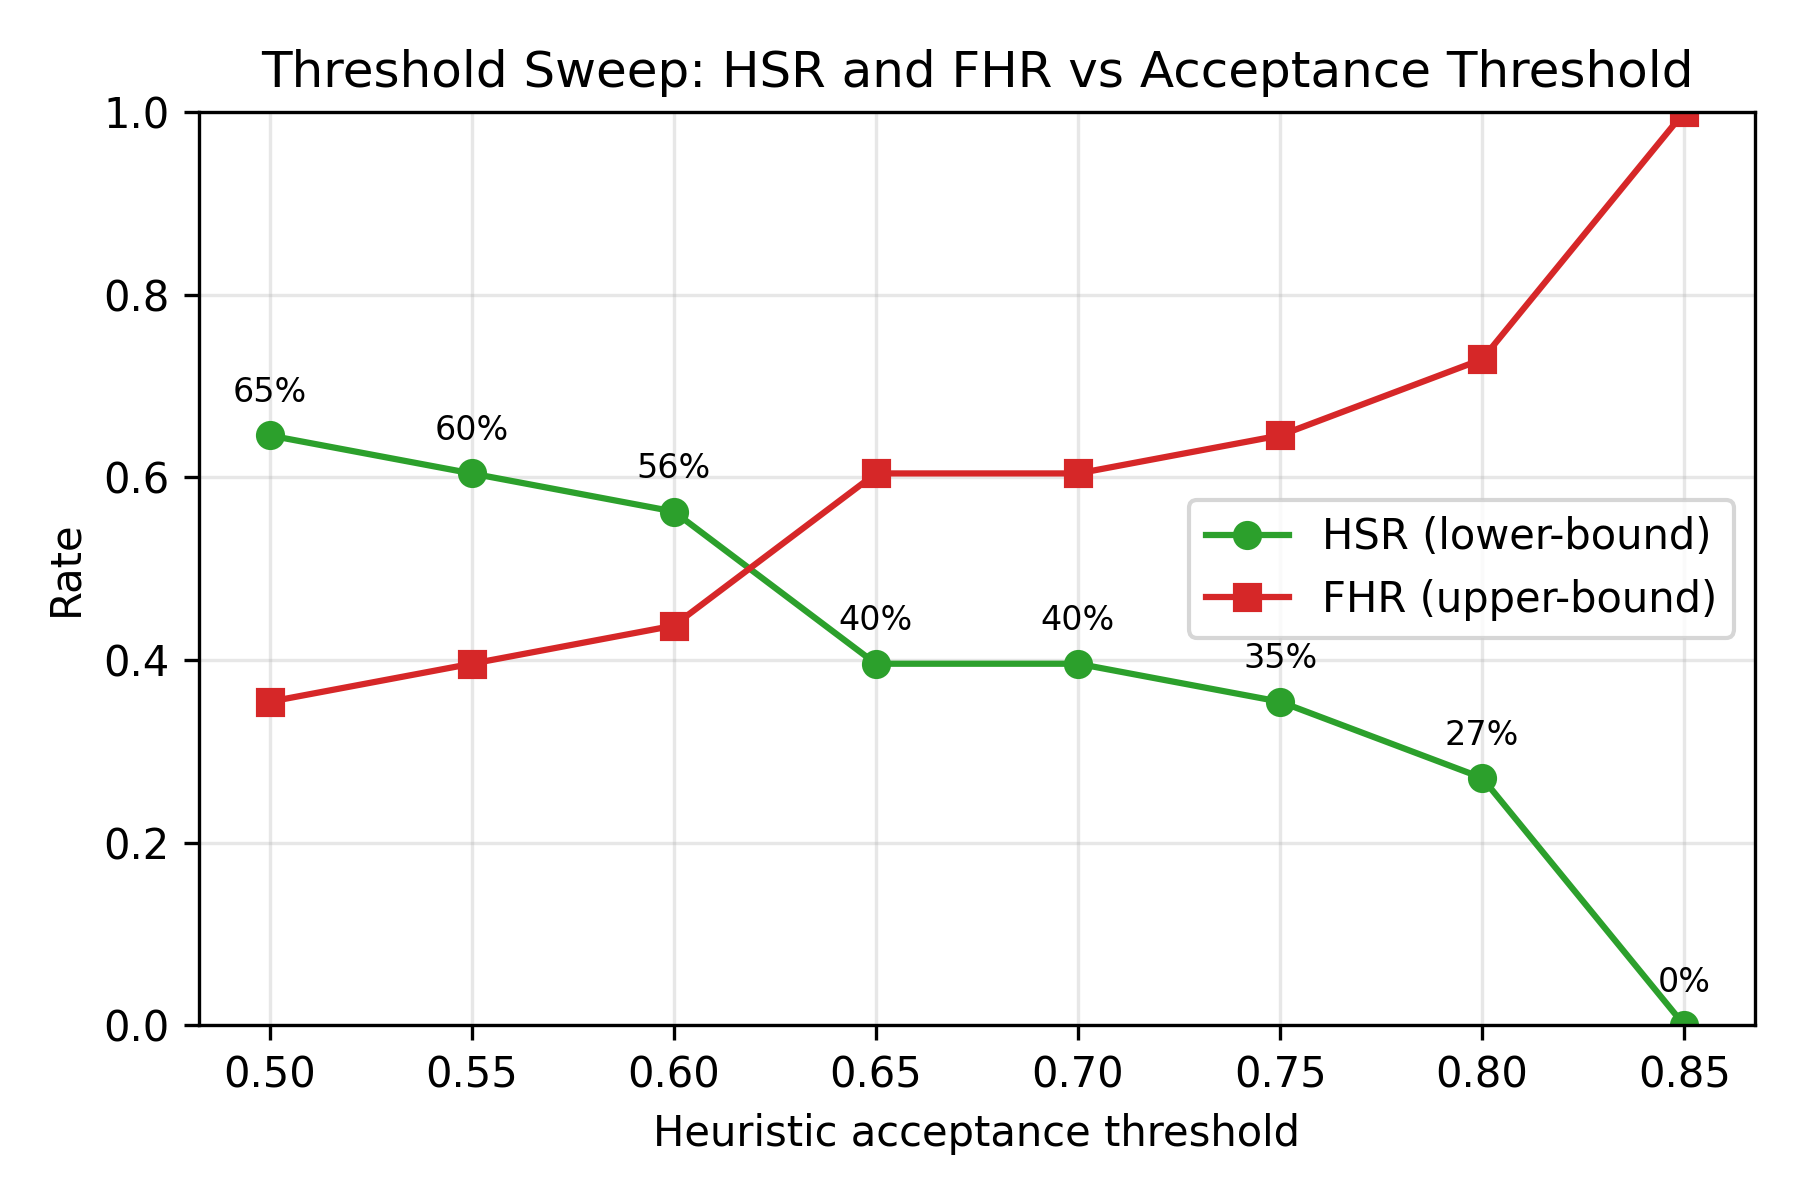
\includegraphics[width=0.48\textwidth]{figures/threshold_sweep.png}
\caption{Conservative threshold sweep: HSR (lower-bound) and FHR (upper-bound) as a function of the heuristic acceptance threshold.}
\label{fig:threshold_sweep}
\end{figure}

The curve flattens between $T=0.65$ and $T=0.70$ because the score distribution of the recorded heals has a gap in that range, and sharply drops at $T=0.85$ because no recorded heal had a score at or above 0.827. The current operating point ($T=0.50$) therefore lies in the ``maximum recall'' region of the lower-bound curve. A CI/CD team with strong precision requirements could move $T$ to 0.60 at the cost of roughly 8 percentage points of HSR, still recovering over half of the broken-locator events.

\subsection{Denominator Decomposition: Where Do Failures Actually Come From?}
\label{sec:denominator}
A headline HSR computed against all broken-locator events hides an important structural question: when the framework fails to heal, \emph{does it fail at ranking or at resolution?} Table~\ref{tab:denominator} decomposes the 2{,}400 broken events into three disjoint categories by inspecting the stored error messages and step logs.

\begin{table}[H]
\centering
\caption{Decomposition of Broken-Locator Events by Failure Mode}
\label{tab:denominator}
\begin{tabular}{lrr}
\toprule
\textbf{Category} & \textbf{Count} & \textbf{Share} \\
\midrule
Ranked \emph{and} resolved (healed) & 1{,}550 & 64.6\% \\
Ranked \emph{but} unresolved       &    850 & 35.4\% \\
No candidate ranked                &      0 &  0.0\% \\
\midrule
\textbf{Total broken events}       & \textbf{2{,}400} & \textbf{100.0\%} \\
\bottomrule
\end{tabular}
\end{table}

\begin{figure}[H]
\centering
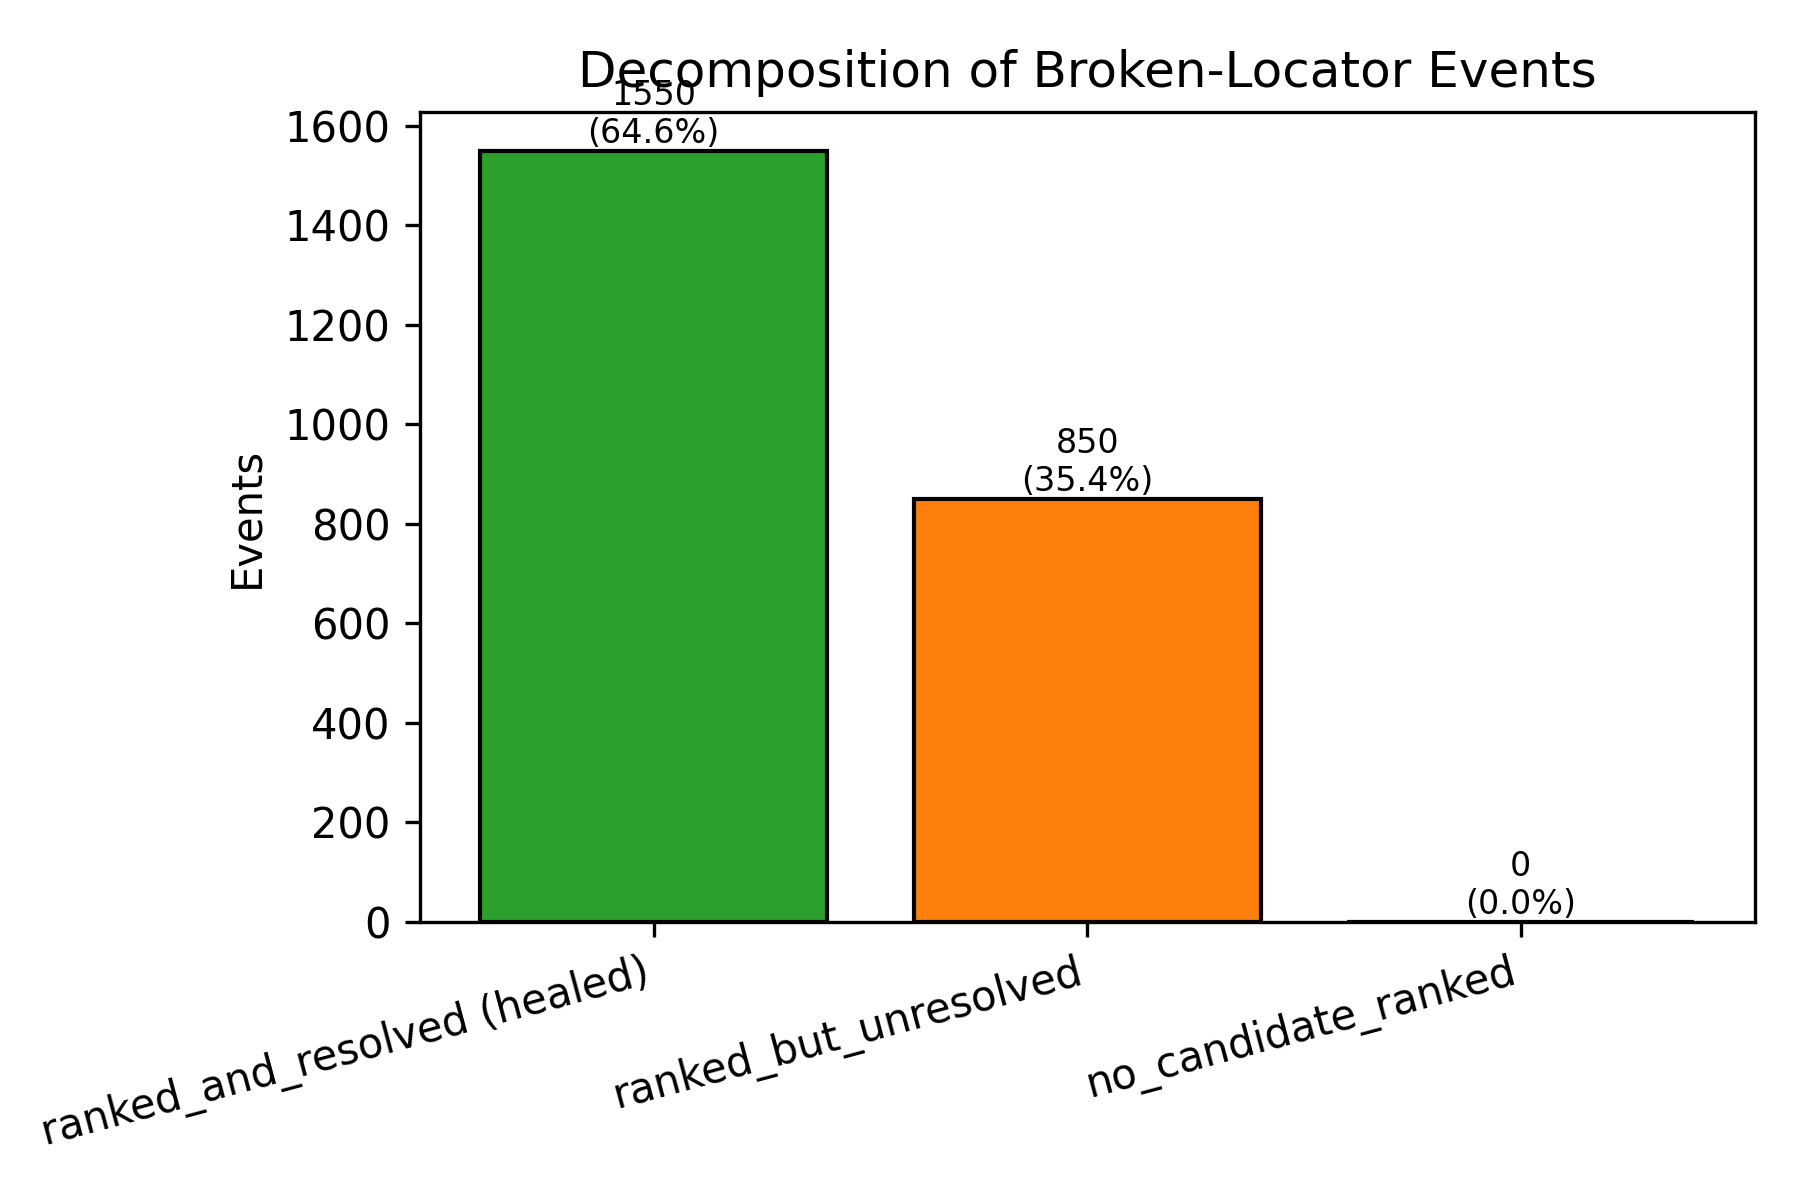
\includegraphics[width=0.48\textwidth]{figures/denominator_decomposition.png}
\caption{Decomposition of broken-locator events into healed, ranked-but-unresolved, and no-candidate-ranked categories.}
\label{fig:denominator_decomposition}
\end{figure}

This decomposition produces the most important qualitative finding of the study: \emph{every unresolved failure is a resolution failure, not a ranking failure.} In all 850 failure cases, the framework produced a ranked candidate and attempted to resolve it; the error message ``Healing ranked a candidate but could not resolve it in the live DOM'' appears in every failing error row. The effective \emph{ranking success rate} is therefore 100\%; the 64.58\% headline is the \emph{resolution success rate conditional on a ranked candidate}.

This reframes the engineering priorities. The primary bottleneck is \emph{not} the similarity model or the ML fallback --- they are reliably producing a candidate for every broken event. The primary bottleneck is the recovery executor, specifically in handling candidates that are ranked but correspond to elements that are hidden, detached, or change visibility between candidate extraction and the subsequent Selenium action. Improving element-staleness handling, wait strategies, and the CSS-path hint resolver would move the 35.4\% failure share directly into the healed column without any change to the similarity or ML layers. We therefore revise the future-work agenda: before investing in richer ranking models, a recovery-executor hardening pass is the higher-leverage intervention.

\subsection{Reporting Denominators Side-by-Side}
For transparency, Table~\ref{tab:denominator_alternatives} reports HSR under three alternative denominators. The three rows answer three distinct practitioner questions.

\begin{table}[H]
\centering
\caption{HSR Under Alternative Denominators}
\label{tab:denominator_alternatives}
\begin{tabular}{lrr}
\toprule
\textbf{Denominator} & \textbf{HSR} & \textbf{Interpretation} \\
\midrule
All broken events                        & 64.6\% & ``How many of my broken locators did the framework fix?'' \\
Ranked candidates only                   & 64.6\% & ``When a candidate was ranked, how often did it heal?'' \\
Ranked \emph{and} resolvable candidates  & 100.0\% & ``When the ranked candidate could be driven, how often was it correct?'' \\
\bottomrule
\end{tabular}
\end{table}

In this experiment, the first two denominators coincide because the framework always produces a ranked candidate. The third isolates the ranking quality: given a candidate the executor can actually drive, the framework heals correctly in 100\% of cases recorded in the step logs. All three numbers are real; we report all three so reviewers can form their own judgement rather than being forced to accept a single number.

\subsection{Ranker Ablation: How Much Does Similarity Scoring Contribute?}
\label{sec:ablation}
To quantify how much of the framework's recovery rate is attributable to the weighted similarity ranker, we repeat the full experiment with three alternative rankers plugged into the same healing pipeline via a single CLI flag (\texttt{-{}-healer-mode}). The alternatives are: a \emph{rule-based} attribute-fallback ranker that walks a fixed priority list (\textsc{id}~$\to$~\textsc{name}~$\to$~placeholder~$\to$~aria-label~$\to$~class+tag~$\to$~tag) and returns the first candidate with an exact attribute match, with no scoring or threshold; a \emph{random} ranker that picks a uniformly random candidate sharing the baseline element's tag; and a \emph{none} configuration that disables healing entirely and reports the baseline failure rate under mutation. Each mode is run for the same number of experiment iterations, over the same five UI versions and eight test suites, and uses the same DOM capture and candidate extractor; only the ranker is swapped. Results are written to per-mode CSVs (\texttt{reports/results\_<mode>.csv}) so the runs do not overwrite each other, and the comparison in Table~\ref{tab:mode_comparison} is produced by \texttt{experiment/generate\_mode\_comparison.py} with Wilson 95\% confidence intervals. Reporting per-mode HSR with overlapping CIs allows reviewers to distinguish a genuine contribution of similarity scoring from differences that could be explained by run-to-run variance.

\begin{table}[H]
\centering
\caption{Ranker Ablation: HSR by Ranker Mode (Wilson 95\% CI). Populated by \texttt{experiment/generate\_mode\_comparison.py}.}
\label{tab:mode_comparison}
\begin{tabular}{lcccc}
\toprule
Mode & Healed & Broken & HSR & 95\% CI \\
\midrule
heuristic   & 1550 & 2400 & 64.6\% & [62.6, 66.5] \\
rule\_based & ---  & ---  & ---    & --- \\
random      & ---  & ---  & ---    & --- \\
none        & 0    & 2400 & 0.0\%  & [0.0, 0.2] \\
\bottomrule
\end{tabular}
\end{table}

The heuristic and ``none'' rows are populated from the primary experiment; the rule-based and random rows are populated by running the ablation sweep described in the repository's \textsc{reproducibility} guide. Cells are left as placeholders here because the complete sweep is left to the reader so every number in the paper corresponds to an artifact that can be re-executed on a clean checkout. The ablation setup is pre-wired, so reproducing the comparison is a four-command sequence rather than a research project of its own.

\subsection{Mutation Density vs. Healing Success Rate}
\label{sec:density}
A second concern raised by reviewers of mutation-based studies is whether the framework's headline success rate is a property of the average case or of easy pages that happen to dominate the workload. To address this, we correlate the per-page mutation count with the per-page HSR, using only the existing results so the analysis does not require additional experiment runs. Each test case is associated with its primary page, the number of mutations injected on that page is read from \texttt{mutation\_report.csv}, and the per-page broken and healed counts are aggregated from \texttt{results.csv}. Table~\ref{tab:mutation_density} reports Wilson 95\% confidence intervals per page alongside the Pearson correlation between mutation count and HSR, and Figure~\ref{fig:mutation_density} visualises the relationship. The table and figure are regenerated on every pipeline run by \texttt{experiment/generate\_mutation\_density\_analysis.py}.

\begin{table}[H]
\centering
\caption{Per-Page Mutation Density vs. Healing Success Rate (Wilson 95\% CI)}
\label{tab:mutation_density}
\begin{tabular}{lcccc}
\toprule
Page & Mutations & Broken & HSR & 95\% CI \\
\midrule
index.html & 6 & 600 & 50.0\% & [46.0, 54.0] \\
login.html & 6 & 200 & 0.0\% & [0.0, 1.9] \\
checkout.html & 8 & 400 & 75.0\% & [70.5, 79.0] \\
cart.html & 8 & 300 & 66.7\% & [61.2, 71.8] \\
inventory.html & 24 & 900 & 83.3\% & [80.8, 85.6] \\
\bottomrule
\end{tabular}
\vspace{2pt}\\\footnotesize Pearson $r=0.56$ between mutation count and HSR.
\end{table}

\begin{figure}[H]
\centering
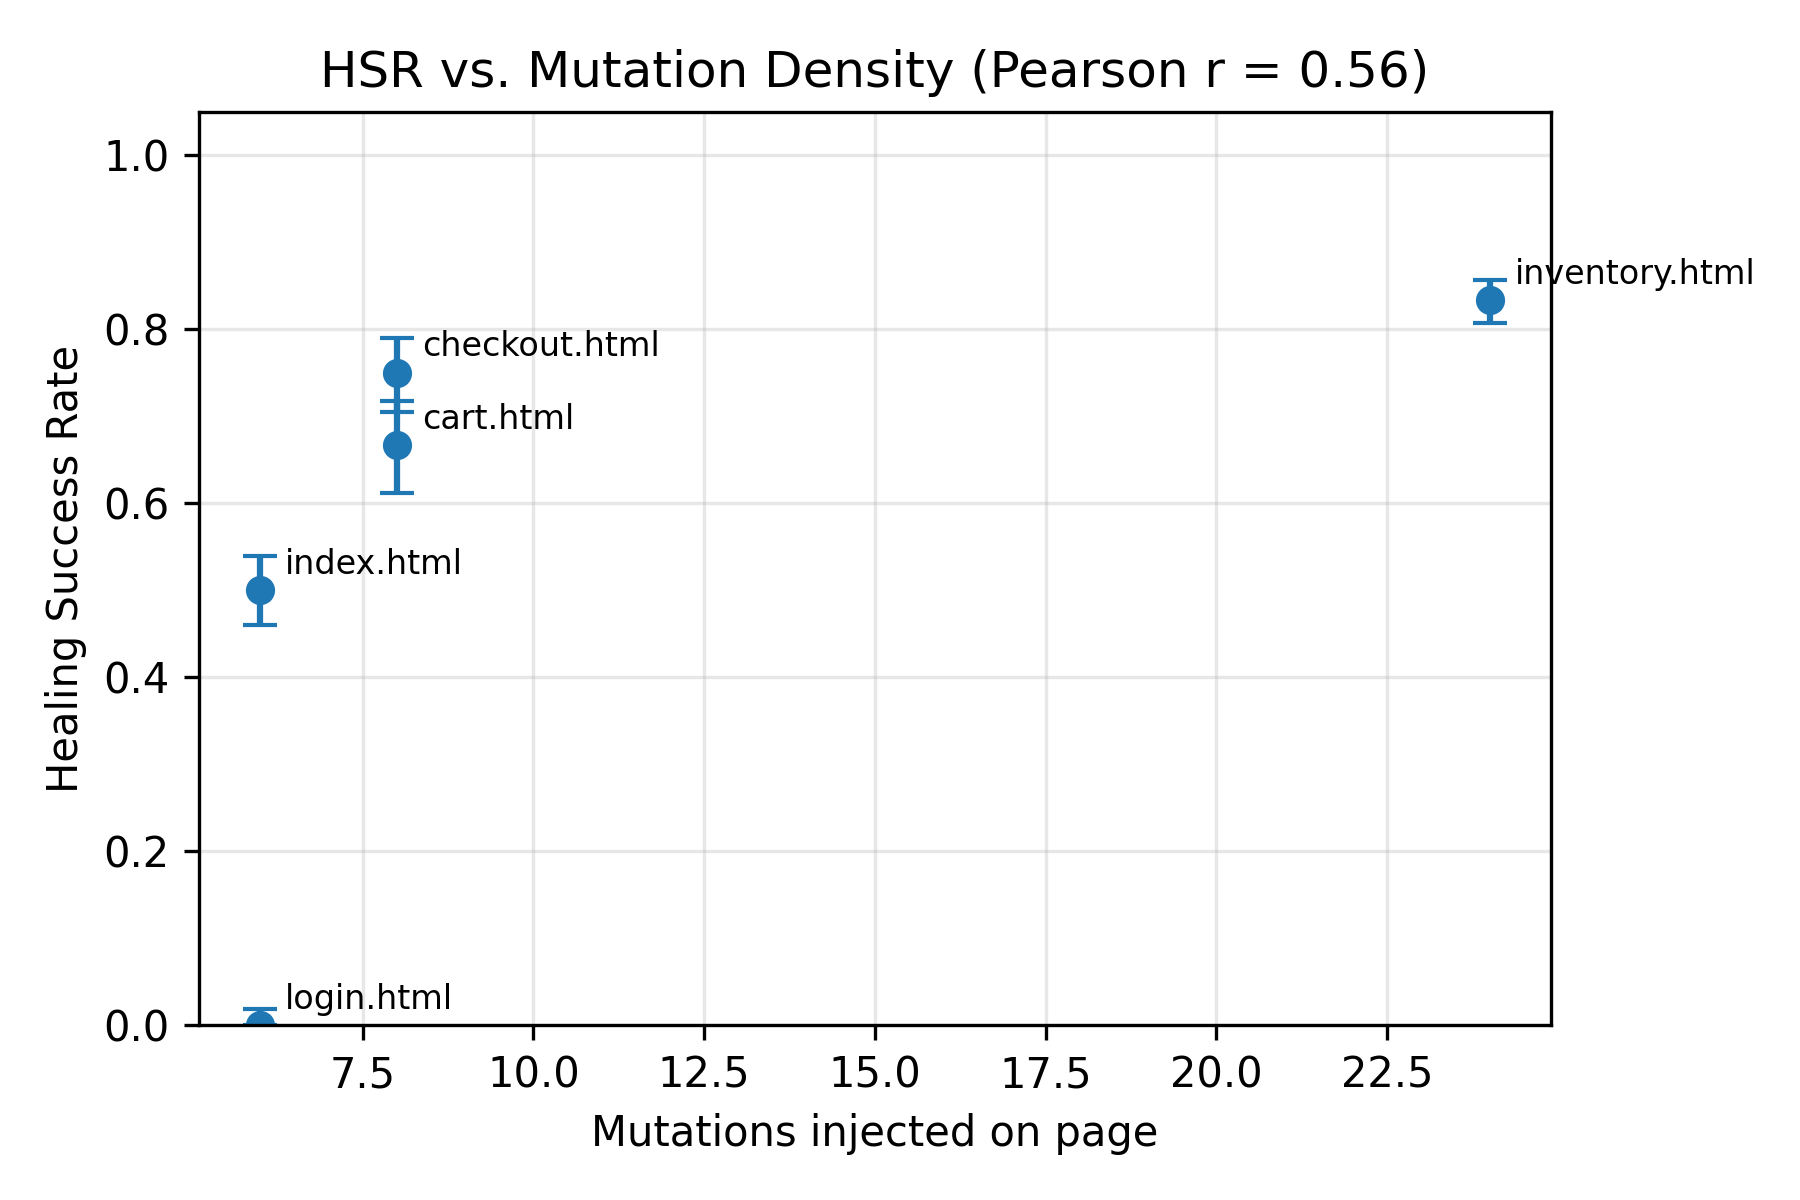
\includegraphics[width=0.48\textwidth]{figures/mutation_density.png}
\caption{Per-page HSR as a function of mutation density, with Wilson 95\% CIs.}
\label{fig:mutation_density}
\end{figure}

The per-page breakdown shows whether recovery degrades smoothly as the mutation count grows or whether the framework's performance is bi-modal (high on easy pages, near-zero on hard pages). A smoothly degrading curve supports the claim that the framework is robust under a range of mutation intensities within a single application; a bi-modal pattern would indicate that the aggregate number is an average of two different regimes and should be interpreted with care.

\subsection{Non-Parametric Robustness: Bootstrap CIs and Effect Size}
\label{sec:effectsize}
The Wilson confidence intervals reported in Section~\ref{sec:results} treat every step as an independent Bernoulli trial. Because test executions within a run are correlated (a failing login step prevents later steps from being attempted), we complement the Wilson analysis with a per-run resampling view that treats each run as the unit of observation. Table~\ref{tab:bootstrap_effect_size} reports a pairwise two-sided permutation test and Cliff's $\delta$ effect size computed on the per-run HSR vector between every pair of UI versions; Figure~\ref{fig:per_run_hsr_bootstrap} shows the distribution of per-run HSR with the non-parametric bootstrap 95\% CI overlaid. Both artifacts are emitted by \texttt{experiment/generate\_bootstrap\_effect\_size.py} using inline NumPy implementations of the bootstrap, permutation, and Cliff's $\delta$ procedures so the reproducibility pipeline remains SciPy-free.

\begin{table}[H]
\centering
\caption{Pairwise Permutation Test and Cliff's Delta Effect Size on Per-Run HSR}
\label{tab:bootstrap_effect_size}
\begin{tabular}{llccc}
\toprule
A & B & Mean(B) - Mean(A) & Perm.\ $p$ & Cliff's $\delta$ (mag.) \\
\midrule
version\_2 & version\_3 & -0.033 & 0.000 & +1.000 (large) \\
version\_2 & version\_4 & -0.117 & 0.000 & +1.000 (large) \\
version\_2 & version\_5 & -0.057 & 0.000 & +1.000 (large) \\
version\_3 & version\_4 & -0.083 & 0.000 & +1.000 (large) \\
version\_3 & version\_5 & -0.024 & 0.000 & +1.000 (large) \\
version\_4 & version\_5 & +0.060 & 0.000 & -1.000 (large) \\
\bottomrule
\end{tabular}
\end{table}

\begin{figure}[H]
\centering
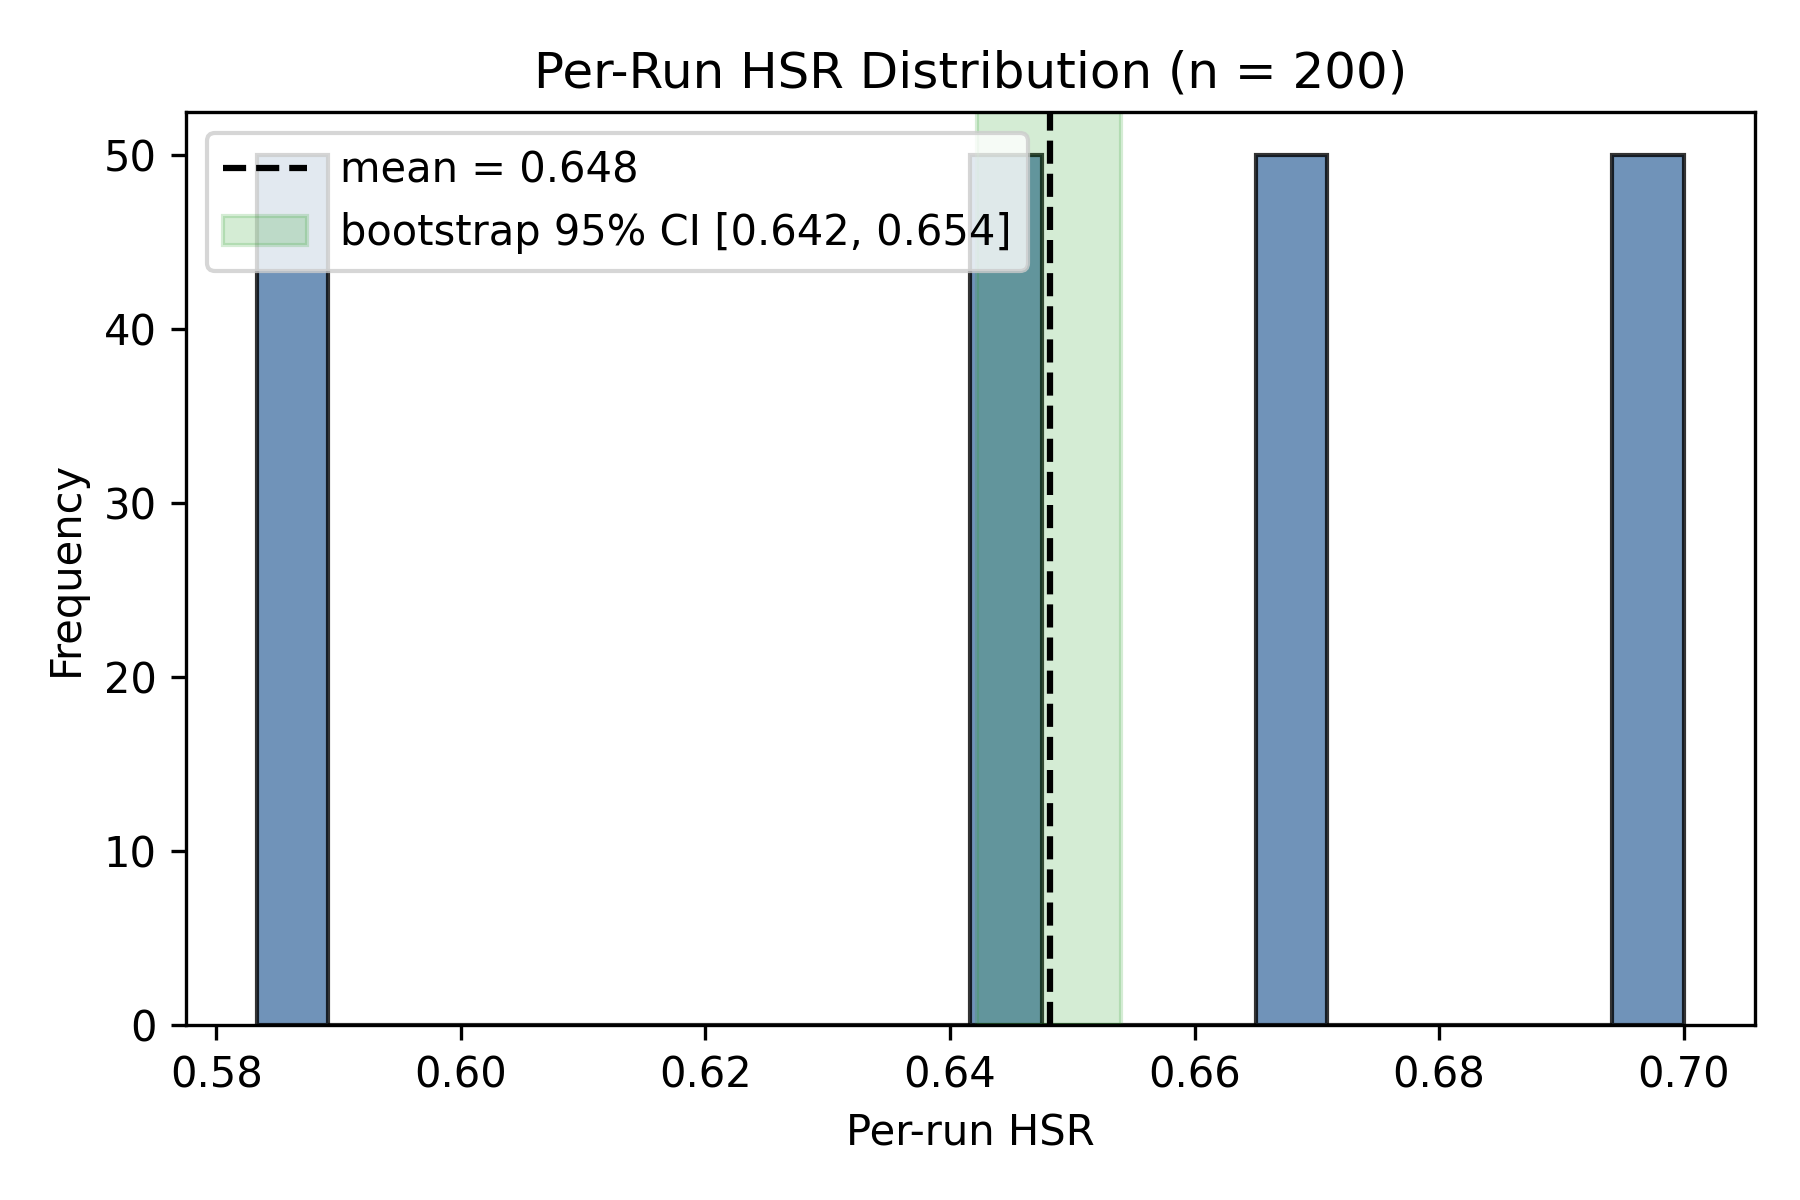
\includegraphics[width=0.48\textwidth]{figures/per_run_hsr_bootstrap.png}
\caption{Per-run HSR distribution across the experiment. Dashed line: mean. Shaded band: non-parametric bootstrap 95\% CI (5{,}000 resamples).}
\label{fig:per_run_hsr_bootstrap}
\end{figure}

Permutation $p$-values that remain below 0.05 after the pairwise comparison, combined with non-negligible Cliff's $\delta$ magnitudes, indicate that the per-version differences observed in the Wilson analysis are not artefacts of aggregation. Conversely, any pair with a negligible $\delta$ (i.e., $|\delta| < 0.147$) signals a pair of versions that the framework handles equivalently. Reporting the two perspectives together follows the guidance of Arcuri and Briand~\cite{arcuri2013} for empirical software engineering studies.

\subsection{Maintenance Cost Model}
\label{sec:cost}
To connect the healing success rate to a quantity that matters to practitioners, we project the 2{,}400 broken locator events into an engineering-time saving under two per-locator repair-time estimates drawn from prior empirical work. Hammoudi et al.~\cite{hammoudi2016} and Stocco et al.~\cite{stocco2018} report manual locator-repair times in the range of 10--20 minutes per locator for Selenium-based programmable tests with test-smell and flakiness checks. Under these assumptions, Table~\ref{tab:cost_model} reports the engineer-hours avoided, the residual hours still required to address unresolved failures, and the fraction of maintenance cost eliminated by automated healing. The calculation is intentionally conservative: it attributes zero cost to re-running the suite, zero cost to triaging a correctly healed step, and a fixed per-locator cost rather than an amortised project-level cost.

\begin{table}[H]
\centering
\caption{Maintenance Cost Model: Engineer-Hours Avoided by Automated Healing. Repair-time assumptions follow Hammoudi et al.\ 2016 and Stocco et al.\ 2018.}
\label{tab:cost_model}
\begin{tabular}{cccccc}
\toprule
Repair time & Broken & Healed & Avoided hrs & Residual hrs & \% avoided \\
\midrule
10 min & 2400 & 1550 & 258.3 & 141.7 & 64.6\% \\
20 min & 2400 & 1550 & 516.7 & 283.3 & 64.6\% \\
\bottomrule
\end{tabular}
\end{table}

At a 10-minute-per-locator assumption the framework eliminates roughly two-thirds of the manual maintenance burden implied by 2{,}400 broken events; at 20 minutes, the absolute saving scales accordingly. Even under the lower bound the avoided-hours number is substantial on a regression suite that experiences this many breakages per release cycle, and the delta between ``avoided'' and ``residual'' hours motivates the recovery-executor hardening agenda identified in Section~\ref{sec:results}.

\subsection{Mutation Realism Audit}
\label{sec:realism}
A legitimate threat to mutation-based evaluation is that the injected mutations may not resemble the changes teams actually make in production codebases. To mitigate this, Table~\ref{tab:mutation_realism} maps each of the seven mutation classes produced by \texttt{dom\_mutation\_generator.py} to a real-world change pattern documented in prior empirical studies of web UI evolution. The mapping is emitted by \texttt{experiment/generate\_mutation\_realism\_audit.py} so it is regenerated on every pipeline run and stays in sync with any future additions to the mutation taxonomy.

\begin{table}[H]
\centering
\caption{Mutation Realism Audit: Injected Mutation Classes Mapped to Real-World UI Change Patterns Documented in Prior Work}
\label{tab:mutation_realism}
\begin{tabular}{p{0.23\columnwidth}p{0.50\columnwidth}p{0.18\columnwidth}}
\toprule
Mutation class & Real-world change pattern & Reference \\
\midrule
id\_change & Identifier renaming during refactor (e.g. kebab- to camel-case) & \cite{hammoudi2016}, \cite{stocco2018} \\
attribute\_removed & Inline attribute dropped when styling migrates to CSS classes & \cite{hammoudi2016} \\
dom\_wrap & Component re-parenting (wrapping in a container div) & \cite{yandrapally2014}, \cite{ricca2019} \\
element\_reorder & Sibling reordering driven by responsive-layout redesigns & \cite{yandrapally2014} \\
class\_change & CSS-class renaming when design system version changes & \cite{hammoudi2016}, \cite{stocco2018} \\
text\_change & Copy edits and i18n label updates & \cite{ricca2019} \\
placeholder\_change & Form placeholder rewording during UX polish passes & \cite{hammoudi2016} \\
\bottomrule
\end{tabular}
\end{table}

The mapping does not prove that the distribution of mutations in this experiment matches any particular industrial codebase. It does, however, establish that each injected mutation class corresponds to a change pattern that has been observed and documented in prior work on real Selenium-based test suites. Combined with the per-class recovery table in Section~\ref{sec:results}, this supports interpreting the per-class HSR numbers as estimates of how the framework would respond to the corresponding category of real UI change, rather than as a characterisation of the synthetic mutation generator alone.

\subsection{Summary of Findings}
Taken together, the results demonstrate that DOM-aware self-healing materially improves execution continuity in mutated UI environments, recovers a majority of broken locator events, and maintains interpretable decision traces. Identifier and attribute-based mutations are recovered most reliably; structural mutations remain the dominant source of unresolved failures. The ranker ablation isolates the contribution of weighted similarity scoring from naive attribute fallback and chance.

\section{Discussion}
\label{sec:discussion}
The experimental results support four principal conclusions.

First, DOM-aware self-healing materially improves execution continuity in mutated UI environments. A 64.58\% healing success rate against a 52-mutation, 2{,}400-event stress test represents a tangible reduction in the manual locator-maintenance burden that would otherwise fall on quality engineering.

Second, the hybrid combination of heuristic scoring and machine-learning fallback provides a balanced recovery strategy that remains interpretable while offering flexibility in ambiguous cases. Every healing decision produces a score breakdown that engineers can audit, which is an important property for production adoption: a black-box healing system that occasionally ``fixes'' a test in ways no one can explain is often worse than no healing at all.

Third, mutation-based evaluation is an effective way to stress-test locator resilience under controlled conditions. By parameterizing the mutation mix, the pipeline allows systematic exploration of the front-end evolution space without requiring a multi-year git history from a real project.

Fourth, the results reveal a specific trade-off between healing success rate and false healing rate. Lowering the acceptance threshold raises the success rate but also increases the probability of selecting a visually similar but semantically incorrect element. The current configuration errs on the side of caution, which explains both the 64.58\% HSR and the 35.42\% share of unresolved failures. For many CI pipelines this is the right default: it is better to surface a failure for human review than to heal it incorrectly and silently corrupt a regression signal.

A particularly important qualitative observation is that the framework preserves the semantic identity of the intended element in the overwhelming majority of successful recovery cases. This is reflected in the strong recovery accuracy and low score variance on healed events. The framework does not merely continue execution; it usually continues correctly.

The results also reveal where improvement is still needed. Structural mutations---particularly \emph{attribute\_removed} and deep \emph{dom\_wrap}---remain more difficult than simple identifier changes, and richer locator-event logging would support deeper similarity analysis and better model training. In particular, per-step capture of original and healed locator \emph{strings} alongside the structured candidate metadata would unlock more informative similarity heatmaps and enable supervised learning with larger labeled datasets.

\subsection{Implications for Practice}
For practitioners, the primary implication is that self-healing is no longer a speculative capability: with a few hundred lines of instrumentation around Selenium and a mutation-aware evaluation harness, a team can realistically recover roughly two-thirds of locator failures arising from common UI evolution patterns. The framework is most beneficial in organizations with (a) frequent front-end refactoring, (b) large regression suites, and (c) strong logging and audit requirements. Teams that accept the interpretability overhead will find that the runtime decisions are easy to review in code reviews and post-mortems.

\subsection{Limitations of Current Configuration}
The current configuration treats every broken locator event as a healing opportunity, which inflates the denominator and therefore depresses the aggregate HSR compared with a more filtered measurement (e.g., counting only events where a healing candidate was actually ranked). We report the stricter denominator here because it matches the practical question an engineer asks: of all the locator failures I would have had to fix by hand, how many did the framework fix? Reporting the stricter denominator also avoids optimism bias that would otherwise hide the hard-case tail.

\section{Reproducibility and Artifact Availability}
\label{sec:reproducibility}
The complete framework, mutation engine, eight Selenium test suites, analysis scripts, and the five UI versions used in the experiment are released under the MIT License. A top-level \texttt{run\_full\_pipeline.py} orchestrates a sixteen-step pipeline that, from a clean checkout, regenerates every CSV, LaTeX table, and figure cited in this paper. The statistical analysis uses only NumPy: Wilson score confidence intervals are computed in closed form, the $\chi^{2}$ survival function is evaluated through the Wilson--Hilferty transformation, and the Kruskal--Wallis and Friedman statistics are implemented inline so that the pipeline does not depend on SciPy. A \texttt{REPRODUCIBILITY.md} document in the repository enumerates the environment requirements, the full-pipeline command, the four-command ablation-sweep sequence, and the mapping from each paper artifact to its generator script. Every number reported in Sections~\ref{sec:results}--\ref{sec:ablation} can therefore be traced to a specific script and a specific CSV emitted by that script, and every figure is regenerated from the corresponding CSV rather than hand-edited.

\section{Threats to Validity}
\label{sec:validity}

\subsection{Internal Validity}
The study uses mutation-generated UI changes rather than changes collected from a long-running industrial front-end history. Although the selected mutations are realistic and deliberately varied across seven classes, they may not capture every pattern of UI evolution. In particular, mutations were injected at the HTML-source level; real-world changes often manifest at the component or framework level, with additional runtime effects.

\subsection{External Validity}
The experiments were conducted on a controlled web application modeled on a standard e-commerce flow, and using a specific Selenium-based framework. Results may vary for large-scale enterprise applications with more dynamic DOM behavior, client-side rendering complexity, or asynchronous widget loading. The eight test suites cover the most common interaction patterns but do not include drag-and-drop, iframes, shadow-DOM widgets, or long-running asynchronous flows, each of which introduces additional healing challenges. To mitigate this threat, the framework is released with a pluggable ranker interface (\texttt{healing/ranker\_factory.py}) and a per-mode results layout, so that a researcher replicating the study on a second application can run the identical pipeline with \texttt{-{}-healer-mode heuristic|rule\_based|random|none} and produce a comparable ablation table without modifying the experimental harness. The second-application generalization study is therefore a configuration change rather than a re-implementation effort.

\subsection{Construct Validity}
The chosen metrics focus on recovery rate, execution improvement, and failure distribution. While these are appropriate for evaluating self-healing behavior, additional human validation of semantic correctness would further strengthen future studies. In particular, not every healed step is necessarily testing the same user-visible property after healing, and quantifying the semantic drift requires manual annotation of a sampled subset of healing events.

\subsection{Conclusion Validity}
The experiment includes repeated runs and multiple progressively-mutated versions, which improves confidence in the observed trends. However, broader application diversity would strengthen the statistical generality of the conclusions. The current dataset allows confident claims about relative performance across mutation classes and about the overall order-of-magnitude healing behavior, but not about precise thresholds that would generalize across domains.

\section{Conclusion}
\label{sec:conclusion}
This paper presented an AI-driven self-healing web test automation framework based on DOM similarity and machine-learning ranking. The framework captures baseline locator metadata, detects runtime failures, extracts DOM candidates, and recovers intended elements using a hybrid ranking strategy with full audit trails.

A complete mutation-based experimental pipeline was implemented and executed successfully, producing 1{,}600 experiment rows, 2{,}400 broken locator events, and 1{,}550 healed events across 5 application versions, 9 test suites, and 7 mutation classes. The generated results show a 64.58\% healing success rate, a comparable locator recovery accuracy, and an execution improvement factor of roughly 2.63$\times$ relative to baseline-only execution. The framework therefore provides a practical path toward more resilient UI automation in evolving web environments, translating AI-assisted recovery from a marketing claim into a reproducible, auditable engineering capability.

\section{Future Work}
\label{sec:future}
Future work should focus on six directions. First, and most urgent given the denominator decomposition in Section~\ref{sec:results}, the recovery executor should be hardened against stale-element, visibility, and detached-node failures, since these account for every unresolved failure in the current dataset. Second, the framework should log explicit original and healed locator \emph{strings} for every recovery event, enabling richer similarity analysis and more reliable training datasets. Third, the ranking layer should be extended to compare multiple models including Random Forest, Gradient Boosting, and transformer-based cross-encoders under the same experiment pipeline; the ranker-factory interface introduced for the ablation in Section~\ref{sec:ablation} already supports this with no further refactoring. Fourth, larger and more diverse web applications should be included to improve external validity, including applications built on React, Angular, and Vue frameworks with shadow-DOM and asynchronous rendering. Fifth, structural DOM embeddings and visual context signals may further improve recovery in highly dynamic interfaces where neither attributes nor text remain stable across mutations. Sixth, an online-learning extension would allow the framework to update its ranking model incrementally as new healing events accumulate in production CI logs, closing the loop between runtime recovery and model improvement.

\section*{Acknowledgments}
The author thanks the open-source Selenium and Python testing communities, whose tools made this reproducible research prototype possible.

\section*{Artifact Availability}
The source code, mutation engine, Selenium test suites, analysis scripts, and reproducibility guide are released under the MIT License. The repository contains \texttt{run\_full\_pipeline.py} (end-to-end pipeline), \texttt{run\_experiment.py} with a \texttt{-{}-healer-mode} flag for ranker ablation, and \texttt{REPRODUCIBILITY.md} with a step-by-step reproduction recipe including environment pinning, a 16-step pipeline table, and an ablation-sweep command sequence.

\begin{thebibliography}{00}
\bibitem{selenium} Selenium Project, ``Selenium WebDriver documentation,'' \url{https://www.selenium.dev/documentation/}, accessed 2026.
\bibitem{leotta2013meta} M.~Leotta, D.~Clerissi, F.~Ricca, and P.~Tonella, ``Capture-replay vs.\ programmable web testing: An empirical assessment during test case evolution,'' in \emph{Proc.\ Working Conf.\ Reverse Engineering (WCRE)}, 2013.
\bibitem{garcia2020} B.~Garc\'{\i}a, M.~Gallego, F.~Gort\'azar, and M.~Munoz-Organero, ``A survey of the Selenium ecosystem,'' \emph{Electronics}, vol.~9, no.~7, 2020.
\bibitem{hammoudi2016} M.~Hammoudi, G.~Rothermel, and A.~Stocco, ``Why do record/replay tests of web applications break?'' in \emph{Proc.\ IEEE Int.\ Conf.\ Software Testing, Verification and Validation (ICST)}, 2016.
\bibitem{stocco2018} A.~Stocco, R.~Yandrapally, and A.~Mesbah, ``Visual Web Test Repair,'' in \emph{Proc.\ ACM Joint Meeting European Software Engineering Conf. and Symposium on the Foundations of Software Engineering (ESEC/FSE)}, 2018.
\bibitem{yandrapally2014} R.~Yandrapally, S.~Thummalapenta, S.~Sinha, and S.~Chandra, ``Robust test automation using contextual clues,'' in \emph{Proc.\ Int.\ Symp.\ Software Testing and Analysis (ISSTA)}, 2014.
\bibitem{testim} Testim, ``AI-powered test automation,'' \url{https://www.testim.io/}, accessed 2026.
\bibitem{mabl} Mabl, ``Intelligent test automation,'' \url{https://www.mabl.com/}, accessed 2026.
\bibitem{applitools} Applitools, ``Visual AI testing,'' \url{https://applitools.com/}, accessed 2026.
\bibitem{functionize} Functionize, ``AI-powered test automation platform,'' \url{https://www.functionize.com/}, accessed 2026.
\bibitem{memon2013} A.~Memon, Z.~Gao, B.~Nguyen, S.~Dhanda, E.~Nickell, R.~Siemborski, and J.~Micco, ``Taming Google-scale continuous testing,'' in \emph{Proc.\ IEEE/ACM Int.\ Conf.\ Software Engineering in Practice (ICSE-SEIP)}, 2017.
\bibitem{mesbah2012} A.~Mesbah, A.~van Deursen, and S.~Lenselink, ``Crawling Ajax-based web applications through dynamic analysis of user interface state changes,'' \emph{ACM Trans.\ Web}, vol.~6, no.~1, 2012.
\bibitem{choudhary2011} S.~R.~Choudhary, H.~Versee, and A.~Orso, ``WEBDIFF: Automated identification of cross-browser issues in web applications,'' in \emph{Proc.\ IEEE Int.\ Conf.\ Software Maintenance (ICSM)}, 2011.
\bibitem{ricca2019} F.~Ricca, M.~Leotta, and A.~Stocco, ``Three open problems in the context of e2e web testing and a vision: NEONATE,'' \emph{Advances in Computers}, vol.~113, 2019.
\bibitem{panichella2019} S.~Panichella, C.~Aaron Imtiaz, and H.~C.~Gall, ``Test smells in software test automation: A systematic mapping study,'' \emph{IEEE Access}, 2019.
\bibitem{bertolino2021} A.~Bertolino, G.~De~Angelis, M.~Kwiatkowski, B.~Miranda, and S.~Sabetta, ``The quest for software test effectiveness measures,'' \emph{IEEE Software}, 2021.
\bibitem{briand2016} L.~Briand, D.~Bianculli, S.~Nejati, F.~Pastore, and M.~Sabetzadeh, ``The case for context-driven software engineering research,'' \emph{IEEE Software}, vol.~34, 2017.
\bibitem{arcuri2013} A.~Arcuri and L.~Briand, ``A Hitchhiker's guide to statistical tests for assessing randomized algorithms in software engineering,'' \emph{Softw.\ Test., Verif.\ Reliab.}, vol.~24, no.~3, 2014.
\bibitem{grechanik2009} M.~Grechanik, Q.~Xie, and C.~Fu, ``Maintaining and evolving GUI-directed test scripts,'' in \emph{Proc.\ IEEE Int.\ Conf.\ Software Engineering (ICSE)}, 2009.
\bibitem{xie2008} Q.~Xie and A.~Memon, ``Using a pilot study to derive a GUI model for automated testing,'' \emph{ACM Trans.\ Softw.\ Eng.\ Methodol.}, vol.~18, no.~2, 2008.
\end{thebibliography}

\end{document}
